\documentclass[preprint2,numberedappendix,tighten]{aastex6}  % USE THIS TO MAKE BIB, THEN FORMAT USING EMULATEAPJ
%\documentclass[twocolumn,apj,numberedappendix]{emulateapj}
\shorttitle{Data Analysis Methods for the Detection of the Epoch of Reionization}
\shortauthors{Cheng et al.}

\usepackage{amsmath}
\usepackage{graphicx}
\usepackage[figuresright]{rotating}
\usepackage{natbib}
\usepackage{ctable}
\citestyle{aa}

%		Math Shortcuts from Adrian
%\def\b{\mathbf{b}}
%\def\k{\mathbf{k}}
%\def\r{\mathbf{r}}
%\def\q{\mathbf{q}}
%\def\b{\mathbf{b}}
%\def\kp{\mathbf{k}^\prime}
%\def\kpp{\mathbf{k}^{\prime\prime}}
%\def\V{\mathbb{V}}
%\def\At{\tilde{A}}
%\def\Vt{\tilde{V}}
%\def\Tt{\tilde{T}}
%\def\tb{\langle T_b\rangle}
%\newcommand{\vis}{\mathbf{v}}
\newcommand{\x}{\mathbf{x}}
\newcommand{\C}{\mathbf{C}}
\newcommand{\Chat}{\mathbf{\hat{C}}}
\newcommand{\F}{\mathbf{F}}
\newcommand{\Fhat}{\mathbf{\hat{F}}}
\newcommand{\Q}{\mathbf{Q}}
\newcommand{\I}{\mathbf{I}}
%\newcommand{\xhat}{\hat{\mathbf{x}}}
%\newcommand{\nhat}{\hat{\mathbf{n}}}
%\newcommand{\A}{\mathbf{A}}
%\newcommand{\N}{\mathbf{N}}
%\newcommand{\rhat}{\hat{\mathbf{r}}}
%\newcommand{\khat}{\hat{\mathbf{k}}}
%\newcommand{\btheta}{\boldsymbol \theta}

\newcommand{\cc}[1]{{\color{purple} \textbf{[CC: #1]}}}
\newcommand{\acl}[1]{{\color{red} \textbf{[ACL:  #1]}}}

\begin{document}
\title{Data Analysis Methods for the Detection of the Epoch of Reionization}

\author{
Carina Cheng\altaffilmark{1},
et al.
}


%		Notes	
	
%Reference section with: \ref{sec:Intro}
%Reference equation with: \eqref{eq:eqtest}
%Reference figure with: \ref{fig:figtest}
%Cite paper inside sentence: \citet{ref}
%Cite paper at end of sentence: \citep{ref}
%Cite paper inside a parenthetical sentence: \citealt{ref}

%To compile with references shown, compile in BibTeX once and LaTeX twice


%		Sample Equation Syntax
%\begin{equation}
%\label{eqtest}
%\langle \widetilde{T} (\mathbf{k}) \widetilde{T}^* (\mathbf{k^\prime}) \rangle = (2 \pi)^3 \delta^D (\mathbf{k} - \mathbf{k}^\prime) P(k),
%\end{equation}


\altaffiltext{1}{Astronomy Dept., U. California, Berkeley, CA}
%\altaffiltext{2}{Hubble Fellow}
%\altaffiltext{2}{Radio Astronomy Lab., U. California, Berkeley, CA}
%\altaffiltext{3}{Berkeley Center for Cosmological Physics, Berkeley, CA}
%\altaffiltext{3}{Dept. of Physics and Astronomy, U. Pennsylvania, Philadelphia, PA}
%\altaffiltext{8}{School of Earth and Space Exploration, Arizona State U., Tempe, AZ}

\begin{abstract}
The Epoch of Reionization (EoR) is an uncharted era in our Universe's history during which the birth of the first stars and galaxies led to the ionization of neutral hydrogen in the intergalactic medium. There are many experiments investigating the EoR by tracing the $21$ cm line of neutral hydrogen, a signal which is very faint and difficult to isolate. With a new generation of instruments and a statistical power spectrum detection in our foreseeable future, it has become increasingly important to develop techniques that help maximize sensitivity and validate results. Additionally, it is imperative to understand the trade-offs between different methods and their effects on common power spectrum themes. In this paper, we focus on three major themes --- signal loss, power spectrum error bar estimation, and bias in measurements. We describe techniques that affect these themes using both a toy model and data taken by the 64-element configuration of the Donald C. Backer Precision Array for Probing the Epoch of Reionization (PAPER). \cc{motivate a bit more once the paper is complete}
\end{abstract}

\section{Introduction}
\label{sec:Intro}

By about one billion years after the Big Bang ($z \sim 6$), the very first stars and galaxies are thought to have ionized all the neutral hydrogen that dominated the baryonic matter content in the Universe. This transition period, during which the first luminous structures formed from gravitational collapse and began to emit intense radiation that ionized the cold neutral gas into a plasma, is known as the epoch of reionization (EoR). The EoR is a relatively unexplored era in our cosmic dawn. Its history encodes important information regarding the nature of the first galaxies and the processes of structure formation. Direct measurements of the EoR would unlock powerful information about the intergalactic medium, revealing connections between the smooth matter distribution exhibited via cosmic microwave background (CMB) studies and the highly structured web of galaxies we observe today.

One promising technique to probe the EoR is to target the 21 cm wavelength emission that is emitted by neutral hydrogen via its spin-flip transition. This technique is powerful because it can be observed as a function of redshift --- that is, the wavelength of the signal reaching our telescopes can be directly mapped to a distance from where the emission originated before stretching out as it traveled through expanding space. Tracing the 21 cm line as a function of redshift offers a window into the evolution of ionization, temperature, and density fluctuations during this transformative era.

Although a detection of the EoR remains elusive, there are several radio telescope experiments that have succeeded in using the 21 cm signal from hydrogen to place constraints on the brightness of the EoR. Examples of experiments investigating the mean brightness temperature of the EoR relative to the CMB are the Experiment to Detect the Global EoR Signature (EDGES; \citealt{bowman2010}), the Long Wavelength Array (LWA; \citealt{ellingson_et_al2009}),  the Large Aperture Experiment to Detect the Dark Ages (LEDA; \citealt{greenhill_bernardi2012}), the Dark Ages Radio Explorer (DARE; \citealt{burns2012}), the Sonda Cosmol\'ogica de las Islas para la Detecci\'on de Hidr\'ogeno NeutroSciHi (SCI-HI; \citealt{voytek2014}), the Broadband Instrument for Global HydrOgen ReioNisation Signal (BIGHORNS; \citealt{sokolowski2015}), and the Shaped Antenna measurement of the background RAdio Spectrum (SARAS; \citealt{patra2015}). Radio interferometers which seek to measure statistical power spectra include the Giant Metre-wave Radio Telescope (GMRT; \citealt{paciga_et_al2013}), the LOw Frequency ARray (LOFAR;\citealt{van_haarlem_et_al2013}), the Murchison Widefield Array (MWA; \citealt{tingay_et_al2013}), the 21 Centimeter Array (21CMA; \citealt{peterson_et_al2004}; \citealt{wu2009}), and PAPER (\citealt{parsons_et_al2010}). The Hydrogen Epoch of Reionization Array (HERA), which is currently being built, is a next-generation instrument that aims to combine lessons learned from previous experiments and is forecasted to be able to make a successful high-significance power spectrum detection with an eventual $350$ elements using current analysis techniques (\citealt{deboer_et_al2017}; \citealt{pober_et_al2014}).

The major challenge that faces all 21 cm experiments is isolating a small signal that is buried underneath foregrounds and instrumental systematics that are, when combined, 4-5 orders of magnitude brighter. A clean measurement therefore requires an intimate understanding of the instrument and a rigorous study of data analysis choices. With continual progress being made in the field and HERA on the horizon, it is becoming increasingly important to understand how the methods we choose interact with each other to affect power spectrum results. More specifically, it is imperative to develop techniques and tests that ensure the accuracy and reliability of a potential EoR detection. In this paper, we discuss three themes that are essential to investigate for a robust $21$ cm power spectrum analysis. We also highlight four power spectrum techniques and their trade-offs, traps, and connections to the themes. We first approach the themes from a broad perspective, and then perform a detailed case study using data from the 64-element configuration of PAPER.

This paper is organized as follows. In section 2 we introduce the three themes of our focus, using a toy model to develop intuition for each one. Section 3 presents a case study into each theme using data from the PAPER-64 array, highlighting key changes from \citet{ali_et_al2015} which have led to a revised PAPER-64 power spectrum limit. We conclude in Section 4.

\section{Power Spectrum Themes and Techniques}
\label{sec:Themes}

There are many choices for a data analyst. How can time-ordered measurements be combined? How can the variance of the data be estimated? In what way(s) can the data be weighted to suppress contaminated modes while not destroying an EoR signal? How can the source of a detection be properly identified? Many common techniques, such as averaging data, weighting, bootstrapping, and jackknife testing, address these issues but harbor additional trade-offs. For example, an aggressive filtering method may succeed in eliminating interfering systematics but comes at the cost of losing some EoR signal. A chosen weighting scheme may maximize sensitivity but fail to suppress foregrounds. 

Despite there being many data analysis choices, measuring the statistical $21$ cm power spectrum ultimately requires robust methods for determining accurate confidence intervals and rigorous techniques to identify and suppress systematics.  In this paper, we focus on three $21$ cm power spectrum themes that encapsulate this goal and discuss four techniques that interplay with each other and impact the themes. We will give brief definitions now, and build intuition for each theme in the sections to follow.

\begin{center}
Power Spectrum Themes
\end{center}

A deep understanding of the following three themes is essential for the accuracy and interpretation of a $21$ cm power spectrum result. Stemmed from a re-analysis of PAPER-64 data, we believe these themes serve as an important check-list for a rigorous power spectrum analysis.
\begin{itemize}
\item \textbf{Signal Loss} (Section \ref{sec:SiglossOverview}): As explained in the next section, certain analysis techniques can lead to the loss of the EoR signal. If not corrected for, it could lead to a false non-detection. Computing signal loss has subtle challenges but is crucial to the accuracy of any result.
\item \textbf{Error Bar Estimation} (Section \ref{sec:ErrorOverview}): Confidence intervals on the $21$ cm power spectrum result determine the difference between a detection and a null result, which have two very different implications. Errors can be estimated in a variety of ways, and we will discuss a few of them.
\item \textbf{Bias} (Section \ref{sec:BiasOverview}): There are several possible sources of bias in a visibility measurement that can show up as a detection in a power spectrum, such as bias from noise and foregrounds. A successful EoR detection would also imitate a bias. Proving a bias is EoR may be the most difficult challenge for $21$ cm analyses, as it is crucial to be able to distinguish a detection of foreground leakage, for example, from that of EoR. In this paper we will highlight some sources of bias and discuss ways to mitigate their effects.
\end{itemize}

\begin{center}
Power Spectrum Techniques
\end{center}

The following techniques each have advantages when it comes to maximizing sensitivity and understanding systematics in data. We focus on these techniques because \cc{??}. However, some have limitations, and we will discuss circumstances in which there are trade-offs.
\begin{itemize}
\item \textbf{Fringe-rate filtering:} Fringe-rate filtering is considered an averaging scheme for time-ordered data (\citealt{parsons_et_al2016}), and we explain the trade-offs of filtering in more detail in Section \ref{sec:SiglossOverview}. Broadly, a fringe-rate filter increases the sensitivity of a dataset and reduces the number of independent samples by an amount dependent on the width of the averaging window. However, it can also affect the presence of foregrounds and systematics. 
\item \textbf{Weighting:} A dataset can be weighted to emphasize certain spectral features and minimize others. One particular flavor of weighting is inverse covariance weighting, which is a generalized version of inverse variance weighting that also takes into account data correlations. This weighting has the effect of down-weighting correlated information (i.e. foregrounds) and up-weighting noise-like information (i.e. EoR). However, a challenge of inverse covariance weighting is in accurately describing a covariance matrix that best describes the data. 
\item \textbf{Bootstrapping:} Because theoretical models for covariance matrices are questionable and theoretical error estimation methods rely on assumptions that can be violated by data, applying theoretical errors to a $21$ cm measurement is often avoided. Hence, bootstrapping is a useful method for estimating errors of a dataset from itself. By randomly drawing many samples of the data, we get a sense of its inherent variance, though there are subtleties to consider such as the independence of values in a dataset.
\item \textbf{Jackknife testing:} A resampling technique useful for estimating bias, jackknives can be taken along different dimensions of a dataset to cross-validate results. In particular, null tests can be used to verify whether results are free of systematics (\citealt{keating_et_al2016}).
\end{itemize}

In the next three subsections, we go into each theme in depth, focusing on how power spectrum technique trade-offs affect each. We use a toy data model to develop intuition into why certain analysis choices may be appealing and discuss ways in which they are limited. We highlight problems that can arise regarding each theme and offer suggestions to mitigate the issues. Ultimately, \cc{some kind of summarizing sentence here}.

\subsection{Signal Loss}
\label{sec:SiglossOverview}

In this section we illustrate how signal loss arises in analysis. Signal loss refers to attenuation of the target cosmological signal in a power spectrum estimate. It can arise in a variety of ways in the analysis pipeline, such as fitting a polynomial during spectral calibration, applying a delay-domain filter, or by weighting data by itself. Here we focus on signal loss associated with applying a weighting matrix to data, a loss that can be significant depending on the choice of weighting and one that was previously underestimated in the PAPER-64 analysis.

Driven by the need to mitigate foreground bias, we use a weighting method that succeeds in down-weighting foregrounds. We apply this weighting to data and propagate it into a final estimator using the power spectrum estimation technique of optimal quadratic estimators (OQE; \citealt{liu_tegmark2011}; \citealt{liu_et_al2014b}). Before showing how signal loss can arise when using different weighting matrices, we first summarize OQE as follows.

We begin with our data vector, $\textbf{x}$ which contains our measured visibilities in Jy. It has length ($N_{t}, N_{f}$), where $N_{t}$ is the number of time integrations and $N_{f}$ is the number of frequency channels. Visibilities are measurements of the Fourier transform of the sky along spatial dimensions, and since we are interested in $3$-dimensional Fourier-modes we only need to take one Fourier transform along the line-of-sight dimension. We do this when forming the un-normalized power spectrum estimate $\hat{q}_{\alpha}$:

\begin{equation}
\label{eq:qhat}
\hat{q}_{\alpha} = \frac{1}{2}\textbf{x}^{\dagger}\textbf{R}\textbf{Q}_{\alpha}\textbf{R}\textbf{x},
\end{equation}

\noindent where $\textbf{R}$ is a weighting matrix. As an example, inverse covariance weighting would set $\textbf{R} = \textbf{C}^{-1}$ and an unweighted case would use $\textbf{R} = \textbf{I}$, the identity matrix. The matrix $\textbf{Q}$ is an operator that takes our frequency-domain visibilities and Fourier-transforms them into power spectrum space while also taking into account physical constants such as the Boltzmann constant used to convert Jy to Kelvin. The index $\alpha$ denotes a waveband in $k_{\parallel}$, where $k_{\parallel}$ is the Fourier-dual to frequency under the delay approximation (\citealt{parsons_et_al2012b}).

We normalize our power spectrum estimates using the matrix $\textbf{M}$:

\begin{equation}
\label{eq:phat}
\hat{\textbf{p}} = \textbf{M}\hat{\textbf{q}},
\end{equation}

\noindent where $\hat{\textbf{p}}$ is the normalized estimate of the true power spectrum. We have a choice for $\textbf{M}$. For simplicity in this section we set $\textbf{M} \propto \textbf{I}$, although we explore other cases for the analysis of PAPER-64 data as explained in Section \ref{sec:Bias}

In the next sections, we investigate the effects of weighting matrices on signal loss by experimenting with different matrices $\textbf{R}$ and examine their impact on the resulting power spectra estimate $\hat{\textbf{p}}$. Our ultimate goal in experimenting with weighting is to suppress foregrounds perfectly without destroying an EoR signal.

\subsubsection{Toy Model: Inverse Covariance Weighting}
\label{sec:toymodel}

To build our intuition into how a particular choice of weighting, namely inverse covariance weighting, can lead to signal loss, we use a toy model. We construct a simple dataset that contains 2-dimensional data (representing visibility data with $100$ time integrations and $20$ frequency channels). This model represents realistic dimensions of about an hour of PAPER data which might be used for a power spectrum analysis. We create a mock bright foreground signal, $\textbf{x}_{FG}$, as a complex sinusoid that varies in time and frequency, a simplistic but realistic representation of a single bright source. We also create a mock EoR signal, $\textbf{x}_{EoR}$, as a complex, Gaussian random signal. Our combined data vector is $\textbf{x} = \textbf{x}_{FG} + \textbf{x}_{EoR}$, to which we apply different weighting schemes. The three data vectors are shown in Figure \ref{fig:toy_sigloss1}. 

\begin{figure}
	\centering
	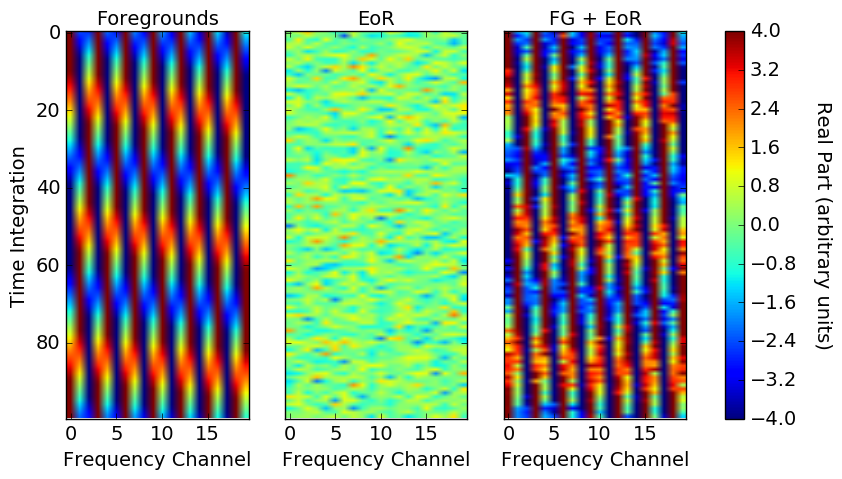
\includegraphics[trim={0.3cm 0.2cm 0.3cm 0.3cm},clip,width=\columnwidth]{plots/toy_sigloss1.png}
	\caption{Our toy model dataset contains a sinusoid foreground that varies in time and frequency and a random Gaussian signal as a mock EoR signal. Real parts are shown here. \cc{colorbar?}}
	\label{fig:toy_sigloss1}
\end{figure}

One choice for a weight matrix $\textbf{R}$ is an inverse covariance matrix. This type of weighting is attractive for power spectrum analyses because it is an aggressive way to down-weight foregrounds and yields the smallest possible error bars on a measurement (\citealt{tegmark_et_al1997a}; \citealt{bond_et_al1998}). The covariance matrix $\textbf{C}$, which in our case describes covariances between frequency channels, can be estimated in a variety of ways. Given perfect foreground, instrumental, and EoR models, we could form $\textbf{C}$ in a way that accurately describes our measured data. However, if our foreground model is flawed for example, our estimate of $\textbf{C}$ would not be successful at down-weighting them in the data.

One attractive way to estimate $\textbf{C}$ is to empirically derive it from the data vector $\textbf{x}$ itself:

\begin{equation}
\hat{\textbf{C}} \equiv \langle\textbf{xx}^{\dagger}\rangle_{t},
\end{equation}

\noindent assuming $\langle\textbf{x}\rangle = 0$, where $\langle \rangle$ denotes a finite average over time $t$. The inverse covariance matrix is therefore $\textbf{R} = \hat{\textbf{C}}^{-1}$. 

First, we compute the power spectrum of $\textbf{x}$ using the OQE formalism and a weighting matrix of $\hat{\textbf{C}}^{-1}$. The result is shown in green in the left plot of Figure \ref{fig:toy_sigloss3}. Also plotted in the figure are the unweighted power spectrum of $\textbf{x}_{FG}$ (blue) and $\textbf{x}_{EoR}$ (red). 

\begin{figure*}
	\centering
	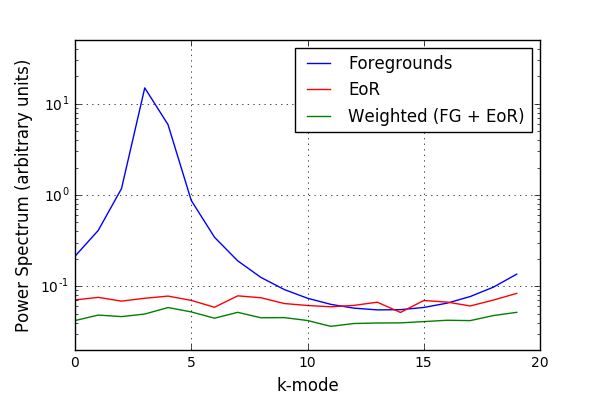
\includegraphics[trim={0.3cm 0.2cm 1cm 0.3cm},clip,height=0.3\textwidth]{plots/toy_sigloss3.png}
	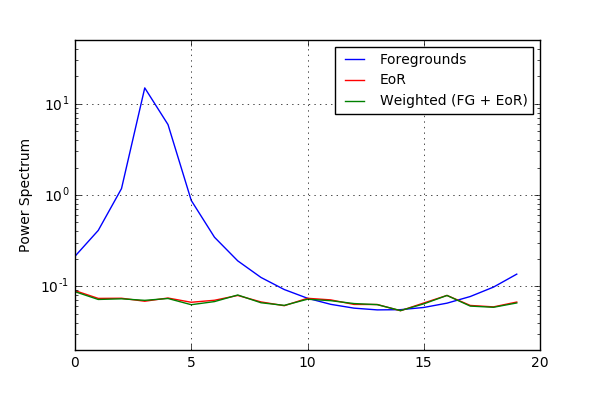
\includegraphics[trim={1cm 0.2cm 0cm 0.3cm},clip,height=0.3\textwidth]{plots/toy_sigloss4.png}
	\caption{Resulting power spectrum estimates for the toy model simulation described in Section \ref{sec:toymodel} --- foregrounds only (blue), EoR only (red), and the weighted FG + EoR dataset (green). We use inverse covariance weighting where $\textbf{C}$ is derived from the data (left), contrasted with projecting out the first eigenmode only (right). In the former case, signal loss arises from using information from all eigenmodes of $\hat{\textbf{C}}$. Because $\hat{\textbf{C}}$ is empirically estimated, its eigenvalues pose the risk of describing random fluctuations that happen to exist in the data realization but may not exist in the true covariance. Consequently, these modes are over-fitted and down-weighted, leading to signal loss. There is no signal loss when using only the zeroth eigenmode, since we are not using information from the weaker eigenmodes which $\hat{\textbf{C}}$ does not describe accurately.}
	\label{fig:toy_sigloss3}
\end{figure*}

As shown, our inverse covariance-weighted result successfully suppresses foregrounds. It is also evident that our result fails to recover the EoR signal --- it exhibits the correct shape, but the amplitude level is slightly low. This is evidence of signal loss. In order to understand the behavior of this result, we need to closely study our covariance matrix, $\hat{\textbf{C}}$, which is shown in Figure \ref{fig:toy_sigloss12}.

\begin{figure}
	\centering
	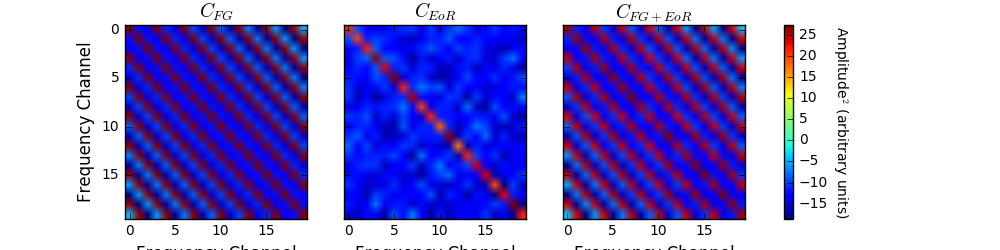
\includegraphics[trim={0.3cm 2.3cm 0.3cm 2.3cm},clip,width=\columnwidth]{plots/toy_sigloss12.png}
	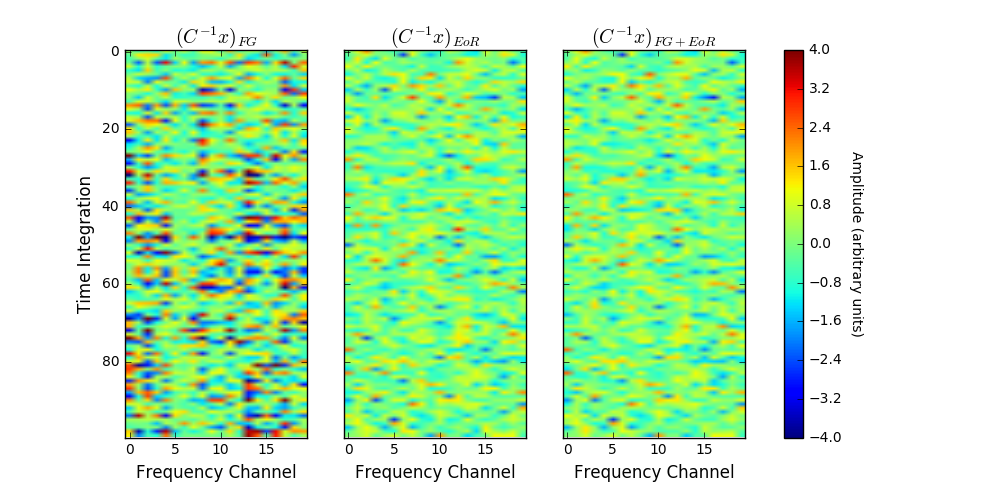
\includegraphics[trim={0.3cm 0.2cm 0.3cm 0.3cm},clip,width=\columnwidth]{plots/toy_sigloss13.png}
	\caption{The covariance matrices (top row) and inverse covariance-weighted data (bottom row) for FG only, EoR only, and FG + EoR. Real parts are shown here. \cc{colorbar?}}
	\label{fig:toy_sigloss12}
\end{figure}

If $\textbf{C}$ is computed from the data itself, it carries the risk of over-fitting information in the data and introducing a multiplicative bias to estimates of the signal. For a mathematical derivation of signal loss arising from a data-estimated covariance matrix, see Appendix \ref{sec:sigloss_appendix}. Here we will describe the origin of this signal loss intuitively.

It turns out that because we estimated $\textbf{C}$ from our data, its eigenspectrum offers insight into understanding how inverse covariance weighting affects our result. An eigenspectrum ranks the eigenvalues of a matrix from highest to lowest and can be thought of as a spectrum of weights that are given to each frequency mode in the data. In other words, the eigenvalues encode the strength of different shapes in the dataset. The eigenspectrum of the identity matrix $\textbf{I}$ is flat (all $1$'s) because it gives equal weighting to all modes. This is usually not the case for a covariance matrix, in which a sloped eigenspectrum means that modes are given different weights. When weighting data by an inverse covariance matrix, the modes with the highest eigenvalues are down-weighted the most. 

\begin{figure}
	\centering
	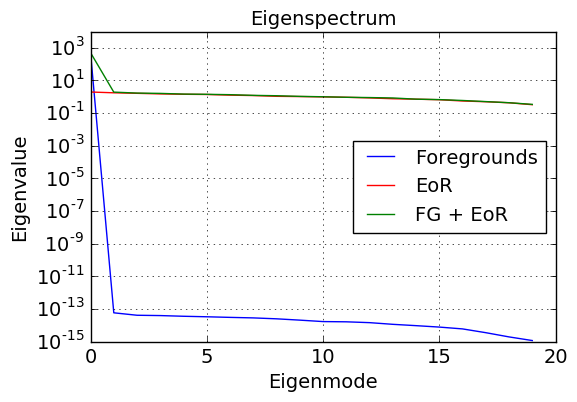
\includegraphics[trim={0.3cm 0.2cm 0.3cm 0.3cm},clip,width=\columnwidth]{plots/toy_sigloss2.png}
	\caption{Eigenspectrum of $\hat{\textbf{C}}_{FG}$ (blue), $\hat{\textbf{C}}_{EoR}$ (red), and $\hat{\textbf{C}}_{FG+EoR}$ (green). The eigenspectrum of $\hat{\textbf{C}}_{FG}$ peaks at the zeroth eigenmode, due to the presence of only one sinusoid.}
	\label{fig:toy_sigloss2}
\end{figure}

If the true covariance matrix $\textbf{C}$ of our data was known, then every single eigenvalue of $\textbf{C}$ would be representative of real fluctuations in the data. However, when using an estimated $\hat{\textbf{C}}$ that is derived from one particular data realization, some of its eigenvalues may be describing random fluctuations that just happen to exist in the data realization. Said differently, shapes that may not exist (or have a weaker existence) in a true covariance may appear stronger in the estimated covariance. Hence, they will be down-weighted more than they should be.

In general, the strongest modes of $\hat{\textbf{C}}$ (highest eigenvalues) are more trustworthy than the weakest modes. Bright foregrounds usually dominate and would therefore exist in both $\textbf{C}$ and $\hat{\textbf{C}}$. This is demonstrated in the toy model by the successful suppression of the foreground mode, where our estimated covariance matrix identifies the sinusoid and assigns it the highest eigenvalue (the peak in Figure \ref{toy_sigloss2}. 

The danger of an empirically estimated covariance matrix comes from not being able to describe weak eigenmodes accurately. The weak eigenmodes of $\hat{\textbf{C}}$ may characterize random noise fluctuations which will be down-weighted. This is what we call the `overfitting' of noise, which leads to signal loss. 

Using what we've learned about the eigenspectrum, we can tweak it in a simple way to suppress foregrounds and yield zero signal loss. Namely, we can project out the zeroth eigenmode (i.e. zero out all eigenmodes except the first one), thereby down-weighting the foregrounds perfectly and nothing else. Hence, we are not using information from all the weaker eigenmodes which carry the risk of describing fluctuations that may not exist in the true covariance. Altering $\hat{\textbf{C}}$ in this way is one example of a regularization method, in which we are changing $\hat{\textbf{C}}$ in a way that flattens its eigenspectrum, making it more identical to that of $\textbf{I}$. The resulting power spectrum estimate for this case is shown in the right plot of Figure \ref{fig:toy_sigloss3}. In this case we recover EoR, demonstrating that if we can model our foregrounds, we can down-weight them without signal loss. There are several other ways to regularize $\hat{\textbf{C}}$, and we will discuss some in Section \ref{sec:otherweight}.

\subsubsection{Toy Model: Fringe-Rate Filtering}

We have shown how signal loss can arise due to inaccurately characterizing weak eigenmodes with a data-estimated covariance. We will next show how this effect is exaggerated by reducing the total number of independent samples in a dataset. 

A fringe-rate filter is an analysis technique designed to maximize sensitivity by integrating in time (\citealt{parsons_et_al2016}). Rather than a traditional box-car average, a fringe-rate filter can be designed to up-weight parts of the sky that an instrument is most sensitive to, while down-weighting the opposite. We apply a fringe-rate filter to PAPER-64 data in order to optimally combine our time-ordered measurements. We weight data based on our primary beam sensitivity, yielding a net increase in sensitivity in our measurements.

Because fringe-rate filtering is analogous to averaging in time, it comes at the cost of reducing the total number of independent samples in the data. To mimic this filter, we average every four time integrations of our toy model dataset together, yielding $25$ independent samples in time (Figure \ref{fig:toy_sigloss5}, left). We choose these numbers so that the total number of independent samples is similar to the number of frequency channels --- therefore, our matrices will be full rank. 

The resulting eigenspectra (Figure \ref{fig:toy_sigloss5}, right), as compared to those in Figure \ref{fig:toy_sigloss2}, fall more steeply, especially for the last few eigenmodes. This is because we have fewer independent modes --- fewer shapes in the data --- so we do a worse job characterizing the weak eigenmodes. Therefore, there is a more dramatic difference in weighting between the modes and we end up down-weighting random noise-like fluctuations more severely than for the un-fringe-rate filtered case. 

\begin{figure*}
	\centering
	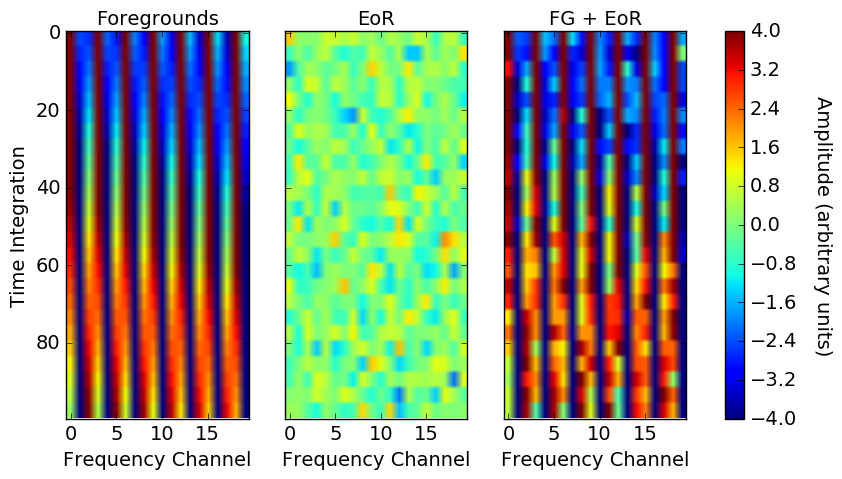
\includegraphics[trim={0.3cm 0.2cm 0.3cm 0.3cm},clip,height=0.3\textwidth]{plots/toy_sigloss5.png}
	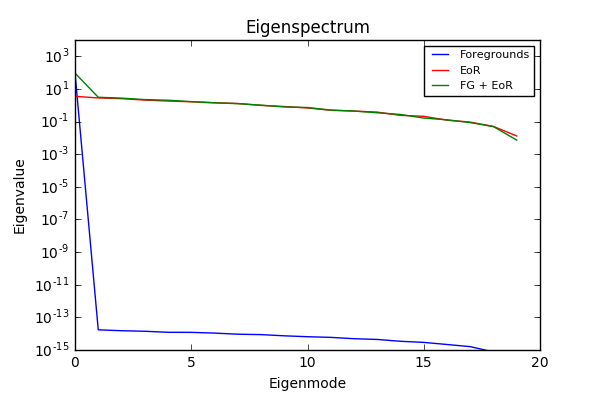
\includegraphics[trim={0.3cm 0.2cm 0.3cm 0.3cm},clip,height=0.3\textwidth]{plots/toy_sigloss6.png}
	\caption{Left: Our `fringe-rate filtered' (time-averaged) toy model dataset. We averaged every four samples together, yielding $25$ independent samples in time. Real parts are shown here. Right: Eigenspectrum of the covariance matrices of foregrounds only (blue), EoR only (red), and FG + EoR (green). The eigenspectrum of foregrounds only peaks at the zeroth eigenmode, a consequence of the presence of only one sinusoid. This spectrum is steeper than that in Figure \ref{fig:toy_sigloss2}, resulting in more dramatic difference in weighting between eigenmodes. Consequently, if all eigenmodes are used in weighting it is possible to down-weight random noisy modes more severely than for the un-fringe-rate filtered case.}
	\label{fig:toy_sigloss5}
\end{figure*}

\begin{figure}
	\centering
	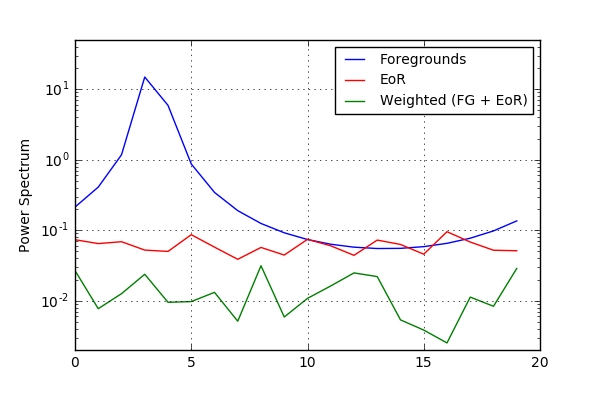
\includegraphics[trim={0.3cm 0.3cm 0.3cm 0.3cm},clip,width=\columnwidth]{plots/toy_sigloss7.png}
	\caption{Resulting power spectrum estimate for the fringe-rate filtered toy model simulation --- foregrounds only (blue), EoR only (red), and the weighted FG + EoR dataset (green). We use inverse covariance weighting where $\textbf{C}$ is derived from the data. There is a larger amount of signal loss than for un-fringe-rate filtered data, a consequence of a steepened, weakly characterized eigenspectrum from using fewer independent modes in the data. This example shows that it is possible to down-weight modes more severely for the un-fringe-rate filtered since there is a more dramatic difference in weighting between modes. The power spectrum estimate is also noisier, since most of the information used in constructing the estimate came from only a few eigenmodes.}
	\label{fig:toy_sigloss7}
\end{figure}

The power spectrum results for inverse covariance weighted fringe-rate filtered data is shown in Figure \ref{fig:toy_sigloss7}. As expected, there is a much larger amount of signal loss for this time-averaged dataset. Additionally, because of the steepened eigenspectrum, most of our power spectrum information is coming from only the last few modes and as a result, it is a noisier estimate. This is evident by noticing that the green curve in Figure \ref{fig:toy_sigloss7} fails to trace the shape of the unweighted EoR power spectrum.

Using our toy model, we have seen that a sensitivity-driven analysis technique like fringe-rate filtering has trade-offs of signal loss and noisier estimates when using data-estimated covariance matrices. Longer integrations increase sensitivity but reduce the number of independent samples, resulting in weakly characterized, steep eigenspectra that can overfit noise greatly.

\subsubsection{Toy Model: Other Weighting Options}
\label{sec:otherweight}

In Section \ref{sec:toymodel} we showed one example of how altering $\hat{\textbf{C}}$ can make the difference between zero and some signal loss, if we can distinguish between real eigenmodes in a true covariance matrix from random fluctuation-induced eigenmodes in an estimated one. We will now use our toy model to describe several other ways to tailor $\hat{\textbf{C}}$ in order to minimize signal loss. We illustrate the resulting power spectra and eigenspectra for four different cases in Figures \ref{fig:toy_sigloss8} and \ref{fig:toy_sigloss14}.

As a first test, we know that our simulated EoR should have a covariance matrix that mimics the identity matrix, with its variance encoded along the diagonal. If we model $\textbf{C}_{EoR}$ as such, instead of computing it based on the dataset itself, and add it to $\hat{\textbf{C}}_{FG} = \langle\textbf{x}_{FG}\textbf{x}_{FG}^{\dagger}\rangle$ to obtain a final $\hat{\textbf{C}}$ to use in weighting, we see that there is negligible signal loss (Figure \ref{fig:toy_sigloss8}, upper left). This is because by modeling $\textbf{C}_{EoR}$, we avoid over-fitting small fluctuations in the data that our model doesn't know about (but an empirically derived $\hat{\textbf{C}}$ would). This is evident when comparing the green and red curves in Figure \ref{fig:toy_sigloss14}. We don't see perfect EoR recovery though, as the green and red curves differ at one $k$ value in Figure \ref{fig:toy_sigloss8}. This deviation is a consequence of the difference between the true and modeled covariance matrices.

\begin{figure*}
	\centering
	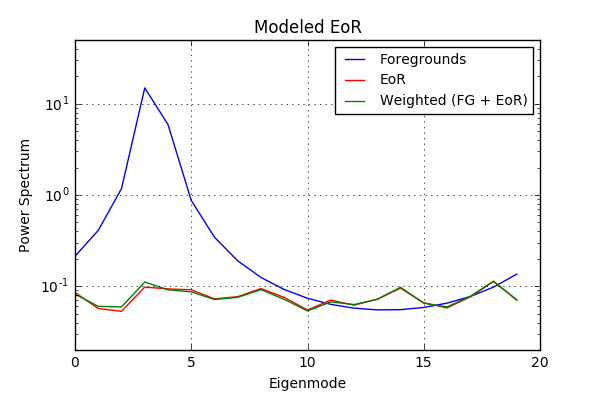
\includegraphics[trim={0.4cm 0.8cm 1.3cm 1cm},clip,height=0.25\textwidth]{plots/toy_sigloss10.png}
	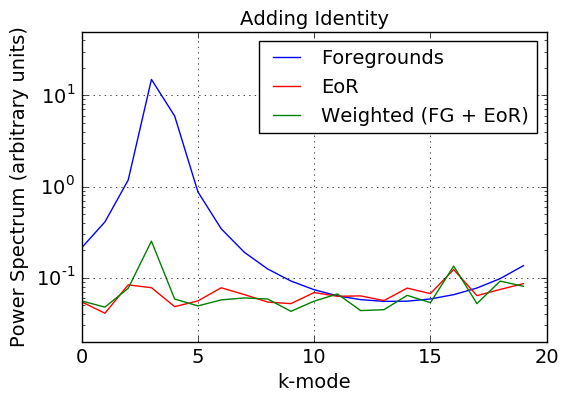
\includegraphics[trim={1cm 0.8cm 1.3cm 1cm},clip,height=0.25\textwidth]{plots/toy_sigloss8.png}
	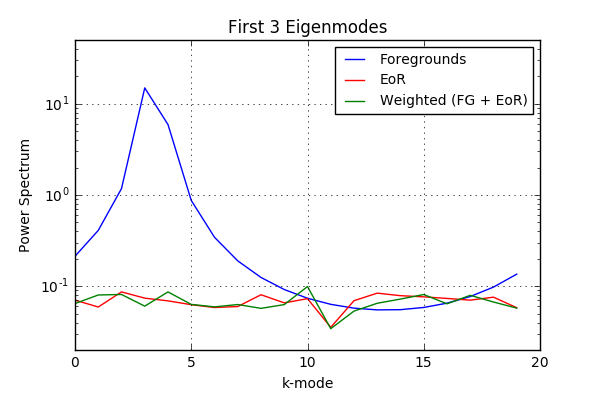
\includegraphics[trim={0.4cm 0.8cm 1.3cm 1cm},clip,height=0.25\textwidth]{plots/toy_sigloss9.png}
	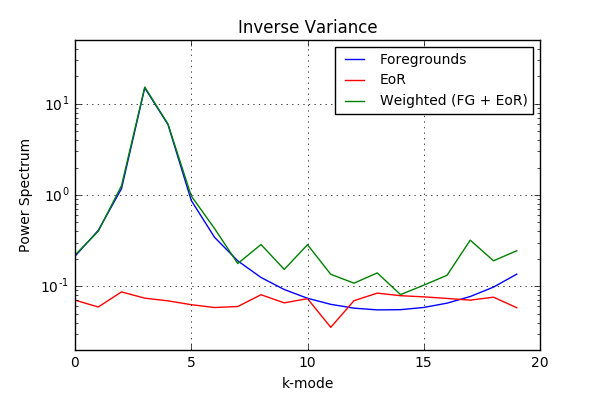
\includegraphics[trim={1cm 0.8cm 1.3cm 1cm},clip,height=0.25\textwidth]{plots/toy_sigloss11.png}
	\caption{Resulting power spectra estimates for our fringe-rate filtered toy model simulation --- foregrounds only (blue), EoR only (red), and the weighted FG + EoR dataset (green). We show four alternate weighting options that each avoid signal loss, including modeling the covariance matrix of EoR (upper left), regularizing $\hat{\textbf{C}}$ by adding an identity matrix to it (upper right), using only the first three eigenmodes of $\hat{\textbf{C}}$ (lower left), and multiplying an identity matrix to $\hat{\textbf{C}}$ (lower right). There are many regularization options available to minimize signal loss, and some work better than others depending on the dataset.}
	\label{fig:toy_sigloss8}
\end{figure*}

\begin{figure}
	\centering
	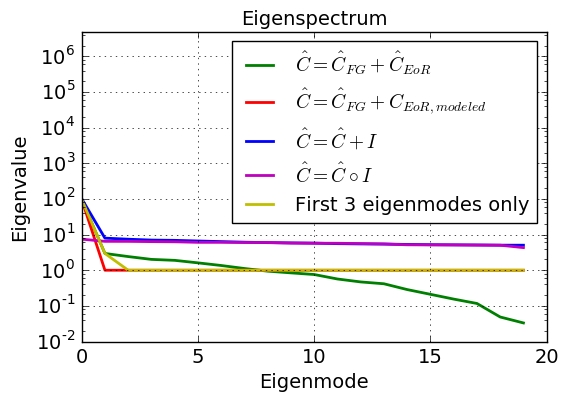
\includegraphics[trim={0.3cm 0.3cm 0.3cm 0.3cm},clip,width=\columnwidth]{plots/toy_sigloss14.png}
	\caption{We compare the eigenspectrum of an empirically calculated $\hat{\textbf{C}}$ (green) to that of four alternate weighting options, including modeling the covariance matrix of EoR (red), regularizing $\hat{\textbf{C}}$ by adding an identity matrix to it (blue), using only the first three eigenmodes of $\hat{\textbf{C}}$ (yellow), and multiplying an identity matrix to $\textbf{C}$ (magenta). }
	\label{fig:toy_sigloss14}
\end{figure}

The second panel (top right) in Figure \ref{fig:toy_sigloss8} uses a regularization method of setting $\hat{\textbf{C}} = \hat{\textbf{C}} + \textbf{I}$. By adding the identity, we are weighting the diagonal elements of the matrix more heavily than those off-diagonal, thereby flattening out its eigenspectrum. If all modes are given similar weights, we avoid down-weighting artificial modes more than others.  

The third panel (bottom left) in Figure \ref{fig:toy_sigloss8} flattens out the eigenspectrum of $\hat{\textbf{C}}$ a different way - by zeroing all but the first three eigenmodes. This means that the first three eigenmodes will be given weights, but the rest will be treated with similar weights. Again, flattening the eigenspectrum results in negligible signal loss. However, we do not perfectly recover the shape of EoR because we lost information when projecting out certain modes. 

The last regularization scheme we are highlighting here is setting $\hat{\textbf{C}} = \hat{\textbf{C}} \cdot \textbf{I}$. In the bottom right panel of Figure \ref{fig:toy_sigloss8}, we see that this method does a poor job down-weighting foregrounds. For this toy model, our foregrounds are spread out in frequency and therefore have non-negligible frequency-frequency correlations. Multiplying by the identity results in a diagonal matrix, meaning we are only left with correlation information between the same two frequencies. Because we disregard information from all other frequency combinations, we do a poor job suppressing the foreground. But because we flattened the eigenspectrum, we also avoid signal loss. 

Although the fourth method did not successfully recover EoR for this particular simulation, it is important that we show that there are many options for estimating a covariance matrix, and some may work better than others based on the dataset. \cc{how to make this paragraph less hand-wavy?} One may imagine a situation where a particular systematic is contained to an isolated frequency. In such a case, preserving only the diagonal elements of $\hat{\textbf{C}}$ would be an effective way of removing this contamination. 

In summary, we have a choice of how to weight $21$ cm data. Ideally, we want to down-weight bright foregrounds without removing the underlying cosmological signal. As we investigated however, there are trade-offs between the weighting method used, its foreground-removal effectiveness, and the amount of resulting signal loss. 

\subsection{Error Estimation}
\label{sec:ErrorOverview}

Our second major $21$ cm power spectrum theme is error estimation, as we desire robust methods for determining accurate confidence intervals for our measurements. Two ways of estimating errors on a power spectrum measurement are calculating the variance of a dataset, and computing a theoretical error estimate based on an instrument's system temperature and observational parameters. In a perfect world, both methods would match up. However, in practice the two don't always agree due to a number of factors, including time, frequency, and antenna-dependent noise and non-uniform weightings. Therefore, it is important to place error bars on our measurements that have been derived from its inherent variance.

A common technique used to estimate the error in a measurement is bootstrapping. Bootstrapping uses sampling with replacement to estimate a posterior distribution. For example, power-spectral measurements of $21$ cm data can be made along many axes, including time and baselines. Through the process of resampling and averaging along these axes, we can estimate error bars for our results which represent the underlying distribution of power spectra values that are allowed by our measurements.

Again, we focus on toy models to highlight traps that one can fall into when bootstrapping power spectra. Suppose we have a Gaussian random signal dataset of length $N=1000$ and unity variance. We are interested in the average of the dataset, and predict that the error on the mean should obey $1/\sqrt{N}$, where $N$ is the number of samples.

We form $100$ bootstraps, each comprised of an array of length $1000$ that is created by a random resampling of the original data, with replacement. The standard deviation over the $100$ bootstraps gives an error estimation for our dataset. As shown in Figure \ref{fig:toy_error1}, the error computed from bootstrapping matches our theoretical prediction.

One major caveat of bootstrapping arises when working with correlated data. If, for example, a dataset has many repeated values inside it, this would be reflected in each bootstrap. The same value would be present multiple times within a bootstrap and also be present between bootstraps, purely because it has a more likely chance of being drawn if there are many of them. Therefore, bootstrapping correlated data results in a smaller variation between bootstraps, and hence, under-estimates errors. The use of a fringe-rate filter, which averages data in time to increase sensitivity, is one example which leads to a reduction in the number of independent samples, creating a situation in which errors can be under-estimated. We will now show this effect using our toy model.

Going back to our toy model, we apply a sliding boxcar average to $10$ samples at a time, thus reducing the number of independent samples to $1000/10 = 100$. Bootstrapping this time-averaged noise, using the same method as described earlier (drawing the same number of samples as the length of the dataset), under-estimates the error by a factor of $\sim3$. This occurs because we are drawing more samples than independent ones available, and thus some samples are repeated multiple times in all bootstraps, leading to less variation between the bootstraps. In fact, the error derived from bootstrapping is a strong function of the number of samples that are drawn (Figure \ref{fig:toy_error1}, black points), and we can both under-estimate the error by drawing too many or over-estimate it by drawing too few. However, if we know that we have $100$ independent samples, the error associated with drawing $100$ samples with replacement does match the theoretical prediction.

This examples highlights the importance of understanding how analysis techniques (e.g. fringe-rate filtering) can affect a common statistical procedure like bootstrapping. Bootstrapping as a means of estimating power spectrum errors from real fringe-rate filtered data requires knowledge of the number of independent samples, which is not always a trivial task. For example, computing the effective number of independent samples of fringe-rate filtered data is not as simple as counting the number of averages performed. Additionally, we can have a non-integer effective number of samples due to the weighting.

\begin{figure}
	\centering
	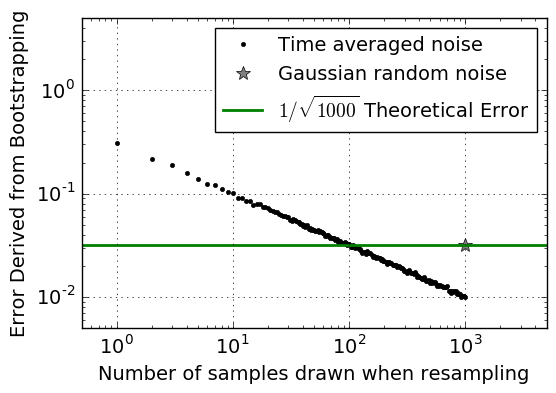
\includegraphics[trim={0.3cm 0.3cm 0.3cm 0.3cm},width=\columnwidth]{plots/toy_error1.png}
	\caption{Error estimation produced by bootstrapping as a function of the number of samples drawn when sampling with replacement. The star represents the error associated with drawing $1000$ samples from a length $1000$ array of a Gaussian random signal. The black points correspond to time-averaged data which has $100$ independent samples. They illustrate how errors can be underestimated if drawing more samples than there are independent samples in the data. The estimated errors match up with the theoretical prediction only at $N=100$.}
	\label{fig:toy_error1}
\end{figure}

We will now discuss a second subtle feature of bootstrapping that can lead to an over-estimation of errors. Suppose we have $5$ independent measurements of the sky (from $5$ different baselines, for example). A bootstrap then consists of $5$ measurements that are drawn randomly with replacement from the original set. If all $5$ spaces are filled randomly, there is a high probability that some measurements will be repeated in the bootstrap because they are drawn more than once. The bootstrap may therefore consist of only $3$ or $4$ independent measurements --- a number smaller than the total number of samples.  In fact, the probability of drawing $5$ completely independent measurements is less than $4\%$.

In order to maximize sensitivity, we desire as many independent samples as possible. However, solely using all $5$ independent measurements does not allow variation between bootstraps. 

Therefore, we use a slightly modified bootstrapping method. For each bootstrap, we first shuffle the data. Next, we take the first $4$ samples, and fill the last slot randomly with replacement. In doing so there is a small chance a bootstrap will consist of $5$ independent samples, but even with $4$ our sensitivity is nearly maximized. One may wonder whether this change is still a legitimate way of error estimating since random sampling only occurs for one value in a bootstrap. However, as long as the number of possible variations is greater than the number of bootstraps we perform, it is a valid way to uncover the inherent variability in a dataset \cc{explain why}. 

In Figure \ref{fig:toy_error2} we compare the two methods of bootstrapping: sampling all elements randomly (black points) versus sampling just the final element randomly (grey points). The two converge for datasets with small numbers of elements, when filling a few spots randomly is nearly the same as filling only the last spot randomly. However, there is also increased scatter in this regime due to small number statistics. 

The difference between the two methods is most pronounced for datasets with large numbers of elements. As a dataset grows in size, it becomes increasingly rare to draw entirely independent samples, and thus the benefit of ensuring, say, $999$ independent samples out of $1000$ is most noticeable. The more elements in our dataset, the more sensitivity we can gain by mandating that most of our measurements are independent ones. An analog for the y-axis in Figure \ref{fig:toy_error2} is therefore the sensitivity of a final power spectrum measurement.

In summary, bootstrapping can be an effective and straightforward way to estimate errors of a dataset. However, we have illustrated two situations in which bootstrapping can lead to inaccurate error estimation. Trade-offs exist between averaging data and the validity of bootstrapping --- working with correlated data gives rise to questions concerning the effective number of independent samples, how to best calculate it, and whether it is valid to simply use that number when bootstrapping. We have also shown a situation in which a naive bootstrapping method can over-estimate errors, thereby compromising measurement sensitivity. While bootstrapping is convenient because it provides a way to estimate errors from the data itself, one must assess whether certain analysis choices have compromised the method and whether a variation of traditional re-sampling could be preferred instead.

\begin{figure}
	\centering
	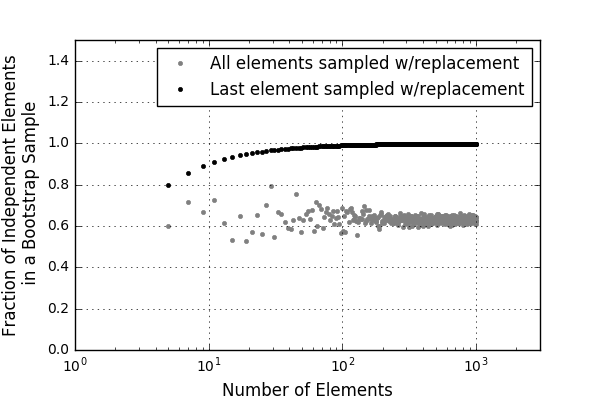
\includegraphics[trim={0.3cm 0.3cm 0.3cm 0.3cm},width=\columnwidth]{plots/toy_error2.png}
	\caption{The fraction of independent elements in a bootstrap as a function of the total number of elements in a dataset. A fraction of $1.0$ means that all elements in a bootstrap are independent, and therefore sensitivity is maximized (alternatively, this axis can be thought of as power spectrum sensitivity). Two bootstrapping methods are shown here --- sampling all elements with replacement (grey) and sampling only the last element with replacement (black). The former over-estimates error bars since some elements end up being repeated due to random sampling. Therefore, sensitivity is not maximized to its full capacity.}
	\label{fig:toy_error2}
\end{figure}

\subsection{Bias}
\label{sec:BiasOverview}

A power spectrum detection could be EoR, but it could also be attributed to other sources of bias. Connecting a detection to EoR as opposed to noise or foreground bias is a key challenge of $21$ cm data analyses. In this section we will discuss possible sources of bias in a measurement, as well as techniques that can help mitigate their effects. We will also present a series of essential tests that a legitimate EoR detection must pass and highlight how these tests can be used to identify biases. These tests serve as a a starting point for the necessary task of verifying a future EoR detection.

\subsubsection{Foreground and Noise Bias}
\label{sec:BiasTypes}

Foreground bias is perhaps one of the main limiting factors pushing up against $21$ cm results. Foreground signals lie $\sim4$-$5$ orders of magnitude above the cosmological signal, and there are many existing techniques to avoid or remove these strong signals. Despite current best efforts to do so, however, there remains some foreground leakage that can show up as detections in a power spectrum. \cc{how do we know that?} 

Because foreground spectra are smooth in frequency, they preferentially show up at low delay, or $k$ modes. For a particular baseline length, there is a maximum delay imposed on foregrounds, which corresponds to the light-crossing time between the two antennas in the baseline. For longer baselines, this value increases, producing what is known as ``the wedge" (\citealt{parsons_et_al2012b}; \citealt{liu_et_al2014a}; \citealt{liu_et_al2014b}; \citealt{vedantham_et_al2012}; \citealt{thyagarajan_et_al2013}). The wedge describes a region in $k$-space contaminated by foregrounds, bounded by baseline length (which is proportional to $k_{\perp}$) and delay (which is proportional to $k_{\parallel}$). Properties of the wedge can be used to isolate and remove foregrounds, as done by \citet{ali_et_al2015}, \citet{parsons_et_al2014}, and \citet{jacobs_et_al2015}.

Despite making power spectrum measurements outside of the wedge in the ``EoR window", foreground detections are still common at low $k$ values. This leakage can be attributed to convolution kernels associated with Fourier-transforming visibilities into delay-space. In other words, smooth-spectrum foregrounds appear as $\delta$-functions in delay-space, convolved by the Fourier transform of the source spectrum and the antenna response, both of which could smear out the foregrounds and cause leakage outside the wedge.

There are analysis techniques to mitigate the effects of foreground leakage and prevent information from low $k's$ from spreading to high $k$ values. For example, narrow window functions can be used to minimize the covariance of a particular $k$ value with other ones (\citealt{liu_et_al2014b}). In other words, one can construct an estimator using OQE that forces a window function to have a minimum response to low $k$ values. The PAPER-64 window function is constructed in such a way, specifically to prevent foregrounds that live at low $k's$ from contaminating higher $k$-modes (see Section \ref{sec:Bias}). Minimizing foreground leakage in this way however, comes with the trade-off of compromising power spectrum sensitivity, since narrow window functions increases errors for each $k$-mode \cc{develop more or cite?}. 

Confirming foreground detections at higher $k$'s is more difficult. In the next section, we will present some tests that can help distinguish these excesses from that of EoR. 

In addition to foreground bias, noise bias can also be responsible for positive power spectrum detections. One example is noise bias arising if thermal noise is multiplied by itself. Every $21$ cm visibility measurement contains thermal noise that is comprised of receiver and sky noise. We expect this noise to be independent between antennas and thus we can beat it down (increase sensitivity) by integrating longer, using more baselines, etc. However, the squaring of noise occurs when cross-multiplying visibilities, which is shown by the two copies of $\textbf{x}$ in Equation \ref{eq:qhat}. If both copies of $\textbf{x}$ come from the same baseline and time, it can result in power spectrum measurements that are higher than those predicted by the thermal noise of the instrument. One way to avoid this type of noise bias is to avoid cross-multiplying data from the same baselines or days. This ensures that the two quantities that go into a measurement have separate noises that don't correlate with each other. 

Another type of noise bias can stem from the spurious cross-coupling of signals between antennas. This excess is known as instrumental crosstalk and is an inadvertent correlation between two independent measurements via a coupled signal path. Crosstalk appears as a constant phase bias in time in visibilities, and it varies slowly compared to the typical fringe-rates of sources. Because it is slow-varying, crosstalk can be suppressed using time-averages or fringe-rate filters. However, there remains a possibility that power spectrum detections are caused by residual, low-level crosstalk which survived any suppression techniques. 

In the next section, we approach the difficult task of tracing excesses to foreground, noise, and EoR biases through a discussion of useful jackknife tests.

\subsubsection{Jackknife Tests}

The jackknife is a resampling technique in which a statistic (i.e. power spectrum) is computed multiple times using subsets of the data. In this section we define two main tests --- the null test and the traditional jackknife --- and explain how a power spectrum detection must pass each. We then highlight how these tests can be used to help distinguish between different sources of bias.
 
\begin{itemize}
\item \textbf{Null Test}: A null test is a type of jackknife test that removes the astronomical signal from data in order to investigate underlying systematics. A clean measurement should be noise-like (a `null' result) if it is not dominated by systematics. There are several ways to perform null tests on data, as implemented in \citet{keating_et_al2016}. For example, one can divide data into two subsets by separating odd and even julian dates, or the first half of the observing season from the second. Subtracting the two removes signal that is common to both subsets, including foregrounds and EoR. The resulting power spectrum should be consistent with thermal noise estimates; if it is not, it suggests the presence of a systematic that differs from one of the data subsets to the other (i.e. doesn't get subtracted perfectly). 
\item \textbf{Traditional Jackknife}: In a more broad sense, it is important to perform many jackknife tests in order to instill confidence in a final result, since a stable result should be consistent through all of them. A successful EoR detection must be steadfast throughout all jackknives no matter how the data is sliced, while other sources of bias may come and go depending on the jackknife performed. Jackknives can be taken along several different axes --- for example, one could start with a full dataset, and compute a power spectrum each time as a day of data is removed, or a baseline is removed. This type of jackknife would reveal bias present only at certain LSTs (such as a foreground source), for example, or misbehaving baselines.
\end{itemize}

While the null test hunts for deviations from thermal noise and the jackknife tests for deviations in subsamples, they are both closely related. We can highlight the connection between the two using a toy model dataset.

Suppose we divide the toy model dataset into two subsets, $\textbf{x}_{1}$ and $\textbf{x}_{2}$, which represent jackknives of the complete dataset $\textbf{x}$.  Both subsets have dimensions of $100$ time integrations and $20$ frequency channels, similar to the toy model used in Section \ref{sec:toymodel}. They also have the same level of thermal noise, constructed as a Gaussian random signal for each. Identical EoR signals, also constructed as a Gaussian random signal, are in both subsets.

The subsets differ in that only one of them contains a foreground signal (a single complex sinusoid) on top of the noise and EoR, representing a bias that only appears for half the data. Mathematically, 

\begin{eqnarray}
\textbf{x}_{1} &=& \textbf{n}_{1} + \textbf{e} + \textbf{fg} \\
\textbf{x}_{2} &=& \textbf{n}_{2} + \textbf{e}
\end{eqnarray}

\noindent where $\textbf{n}$ is noise, $\textbf{e}$ is the EoR signal, and $\textbf{fg}$ is the foreground signal. 

We do not perform a time-average or apply a fringe-rate filter to this toy model, since we are interested only in what jackknife tests can tell us about biases. For the same reason, we use a weighting matrix of $\textbf{I}$ for power spectrum estimation to avoid signal loss. We form $5$ different power spectrum estimates: $\hat{\textbf{p}}$ (full dataset), $\hat{\textbf{p}}_{1}$ (subset $1$), $\hat{\textbf{p}}_{2}$ (subset $2$), $\hat{\textbf{p}}_{noise}$ (noise only), and $\hat{\textbf{p}}_{null}$, which is the result of our differenced dataset $\textbf{x}_{null}$, defined as:

\begin{equation}
\textbf{x}_{null} = \textbf{x}_{1} - \textbf{x}_{2}. 
\end{equation}

\begin{figure}
	\centering
	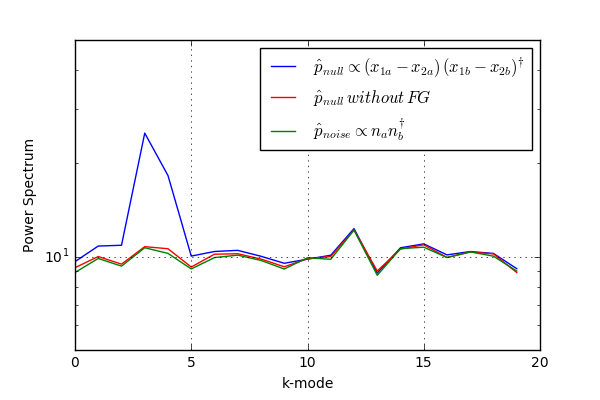
\includegraphics[trim={0.3cm 0.3cm 0.3cm 0.3cm},width=\columnwidth]{plots/toy_bias1.png}
	\caption{Power spectrum estimates for the full toy model dataset $\textbf{x}$ (green), the differenced dataset $\textbf{x}_{1}-\textbf{x}_{2}$, which represents a null jackknife test (black), and noise alone (red). Because $\hat{\textbf{p}}_{null}$ is not consistent with noise, it suggests the presence of a systematic in either $\textbf{x}_{1}$ or $\textbf{x}_{2}$. Null tests of clean measurements should be consistent with thermal noise.}
	\label{fig:toy_bias1}
\end{figure}

\begin{figure}
	\centering
	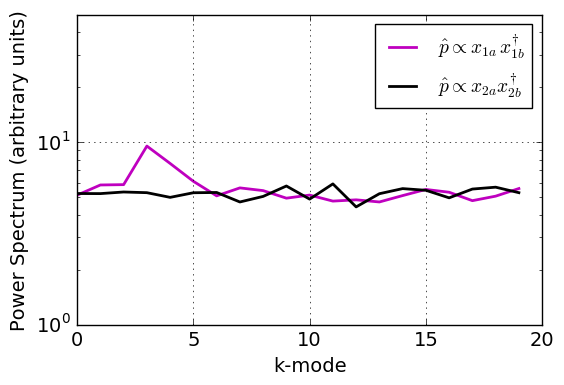
\includegraphics[trim={0.3cm 0.3cm 0.3cm 0.3cm},width=\columnwidth]{plots/toy_bias2.png}
	\caption{Power spectrum estimates for $\textbf{x}_{1}$ and $\textbf{x}_{2}$, two jackknives of the toy model. They suggest the presence of a systematic in $\textbf{x}_{1}$ only, illustrating how jackknives can be used to tease out excesses. Clean measurements should remain consistent despite the jackknife taken.}
	\label{fig:toy_bias2}
\end{figure}

In Figure \ref{fig:toy_bias1}, we compare $\hat{\textbf{p}}_{null}$, $\hat{\textbf{p}}_{noise}$, and $\hat{\textbf{p}}$. Our goal is to determine whether the excess we see in $\hat{\textbf{p}}$ (the power spectrum peak) is due to the EoR signal, something we would not know for a real dataset. The null test reveals that there is also an excess in $\hat{\textbf{p}}_{null}$ --- hence, we can rule out EoR. Because this is a toy model, we know that the excess is attributable to the foreground signal that did not get subtracted off for the null test. 

Additionally, we look at the jackknife results, namely $\hat{\textbf{p}}_{1}$ and $\hat{\textbf{p}}_{2}$. The results are shown in Figure \ref{fig:toy_bias2}. Again, we see a clear difference between the two, signifying a non-EoR bias that is only present in one subset. 

While the null test is useful for ruling out EoR, jackknives are useful in pinpointing which data subsets are contaminated by biases and which are not; in our toy model we see that the bias exists only in $\hat{\textbf{p}}_{1}$. If foreground or noise biases exist in a dataset, jackknives can tease them out and provide insight into possible sources. For example, if jackknives along the time-axis reveal a bias present at a certain LST, a likely explanation would be excess foreground emission from a radio source in the sky at that time. A jackknife test involving data before and after the application of a fringe-rate filter can reveal whether cross-talk noise bias is successfully suppressed with the filter, or if similar-shaped detections in both power spectras suggest otherwise. There are many other jackknife axes of which we will not go into detail here, including baseline, frequency, and polarization. Ultimately, an EoR detection should persist through them all and a clean measurement should pass all null tests. 

In this section we have highlighted how null tests and jackknife tests are key for determining the nature of a power spectrum detection. In Section \ref{sec:Bias} we perform some examples of these tests on PAPER-64 data.

\section{Case Study: PAPER-64}
\label{sec:CaseStudy}

In the previous sections we have discussed three overarching $21$ cm power spectrum themes --- signal loss, error estimation, and bias. Understanding the subtleties and trade-offs involved in each is necessary for an accurate and robust understanding of a power spectrum result. 

We now present a case study of these same three themes using data from the PAPER experiment. We use the intuition we've developed through our toy model simulations in order to make smartly-motivated data analysis choices for PAPER. In light of our new understandings, we also highlight major changes since \citet{ali_et_al2015}.

As a brief review, PAPER is a dedicated $21$ cm experiment located in the Karoo Desert in South Africa. The PAPER-64 configuration consists of 64 dual-polarization drift-scan elements (Figure \ref{fig:paper}) that are arranged in a grid layout. For our case study, we focus solely on Stokes I data from PAPER's $30$ m East/West baselines. For information about the backend system of PAPER-64, its observations, and data reduction pipeline, we refer the reader to \citet{parsons_et_al2010} and \citet{ali_et_al2015}.

\begin{figure}
	\centering
	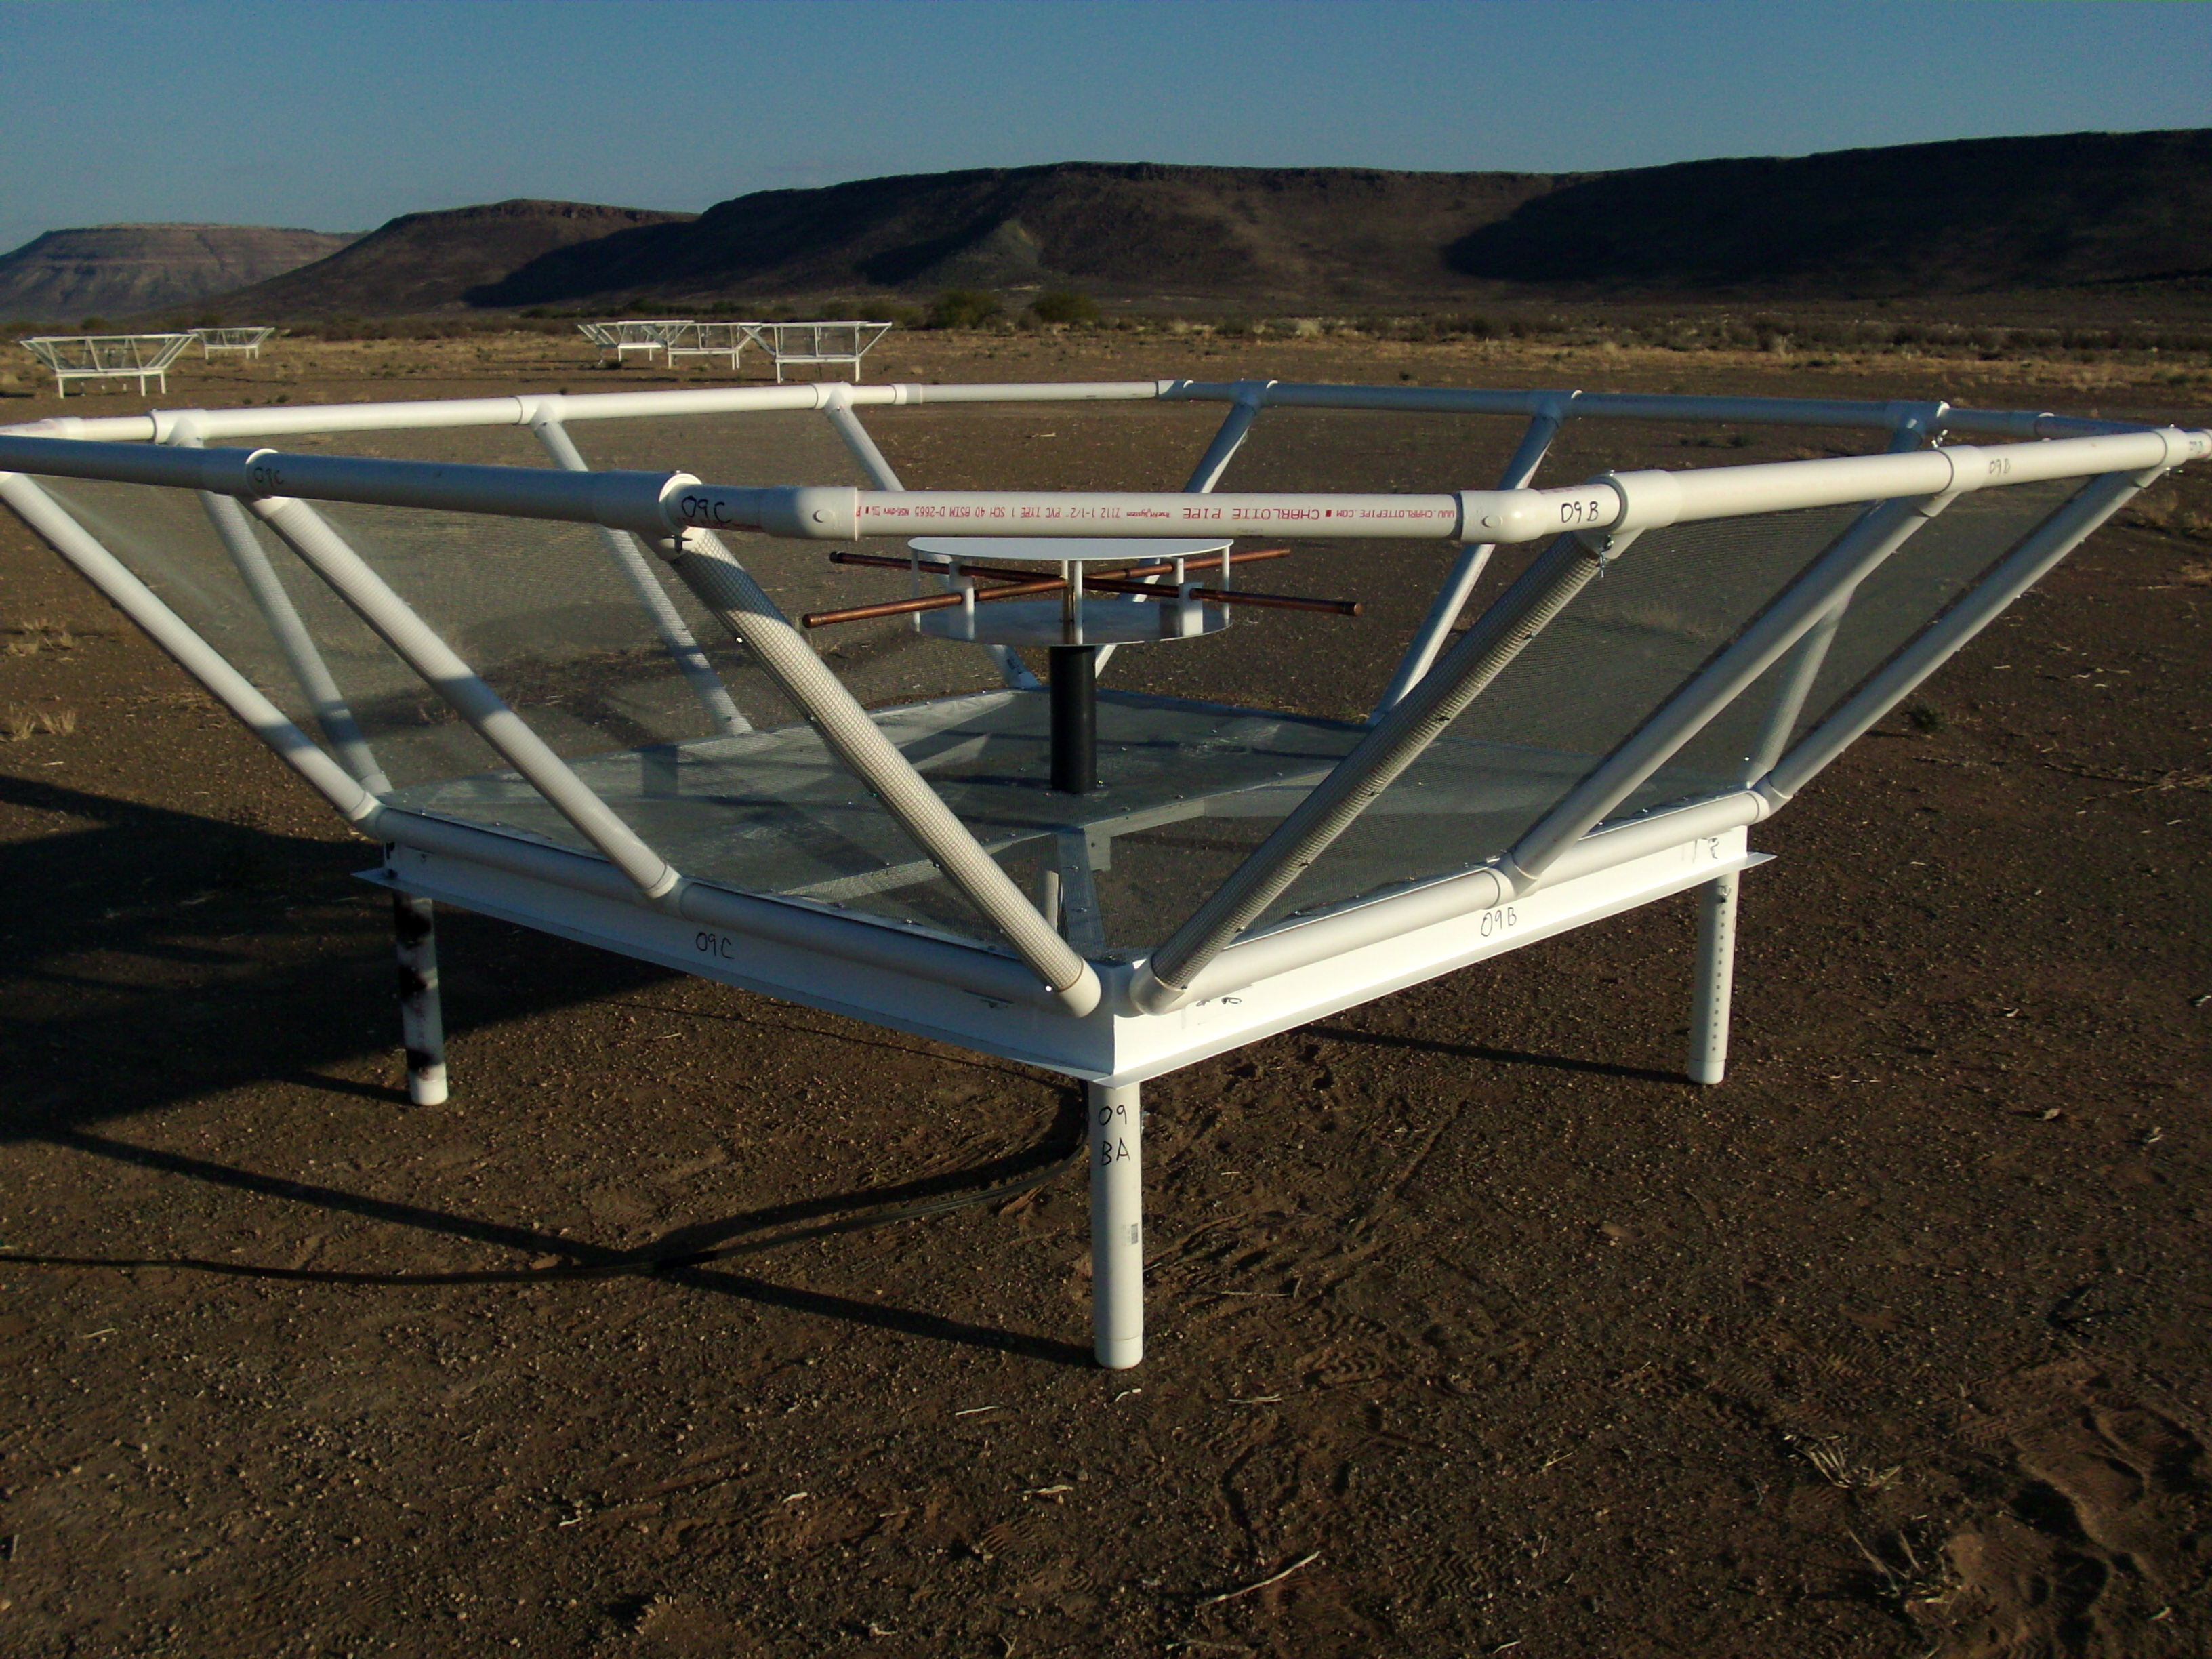
\includegraphics[trim={0.3cm 0.3cm 0.3cm 0.3cm},width=\columnwidth]{plots/paper_dipole.png}
	\caption{PAPER dipole in South Africa.}
	\label{fig:paper}
\end{figure}

%\begin{figure*}
%	\centering
%	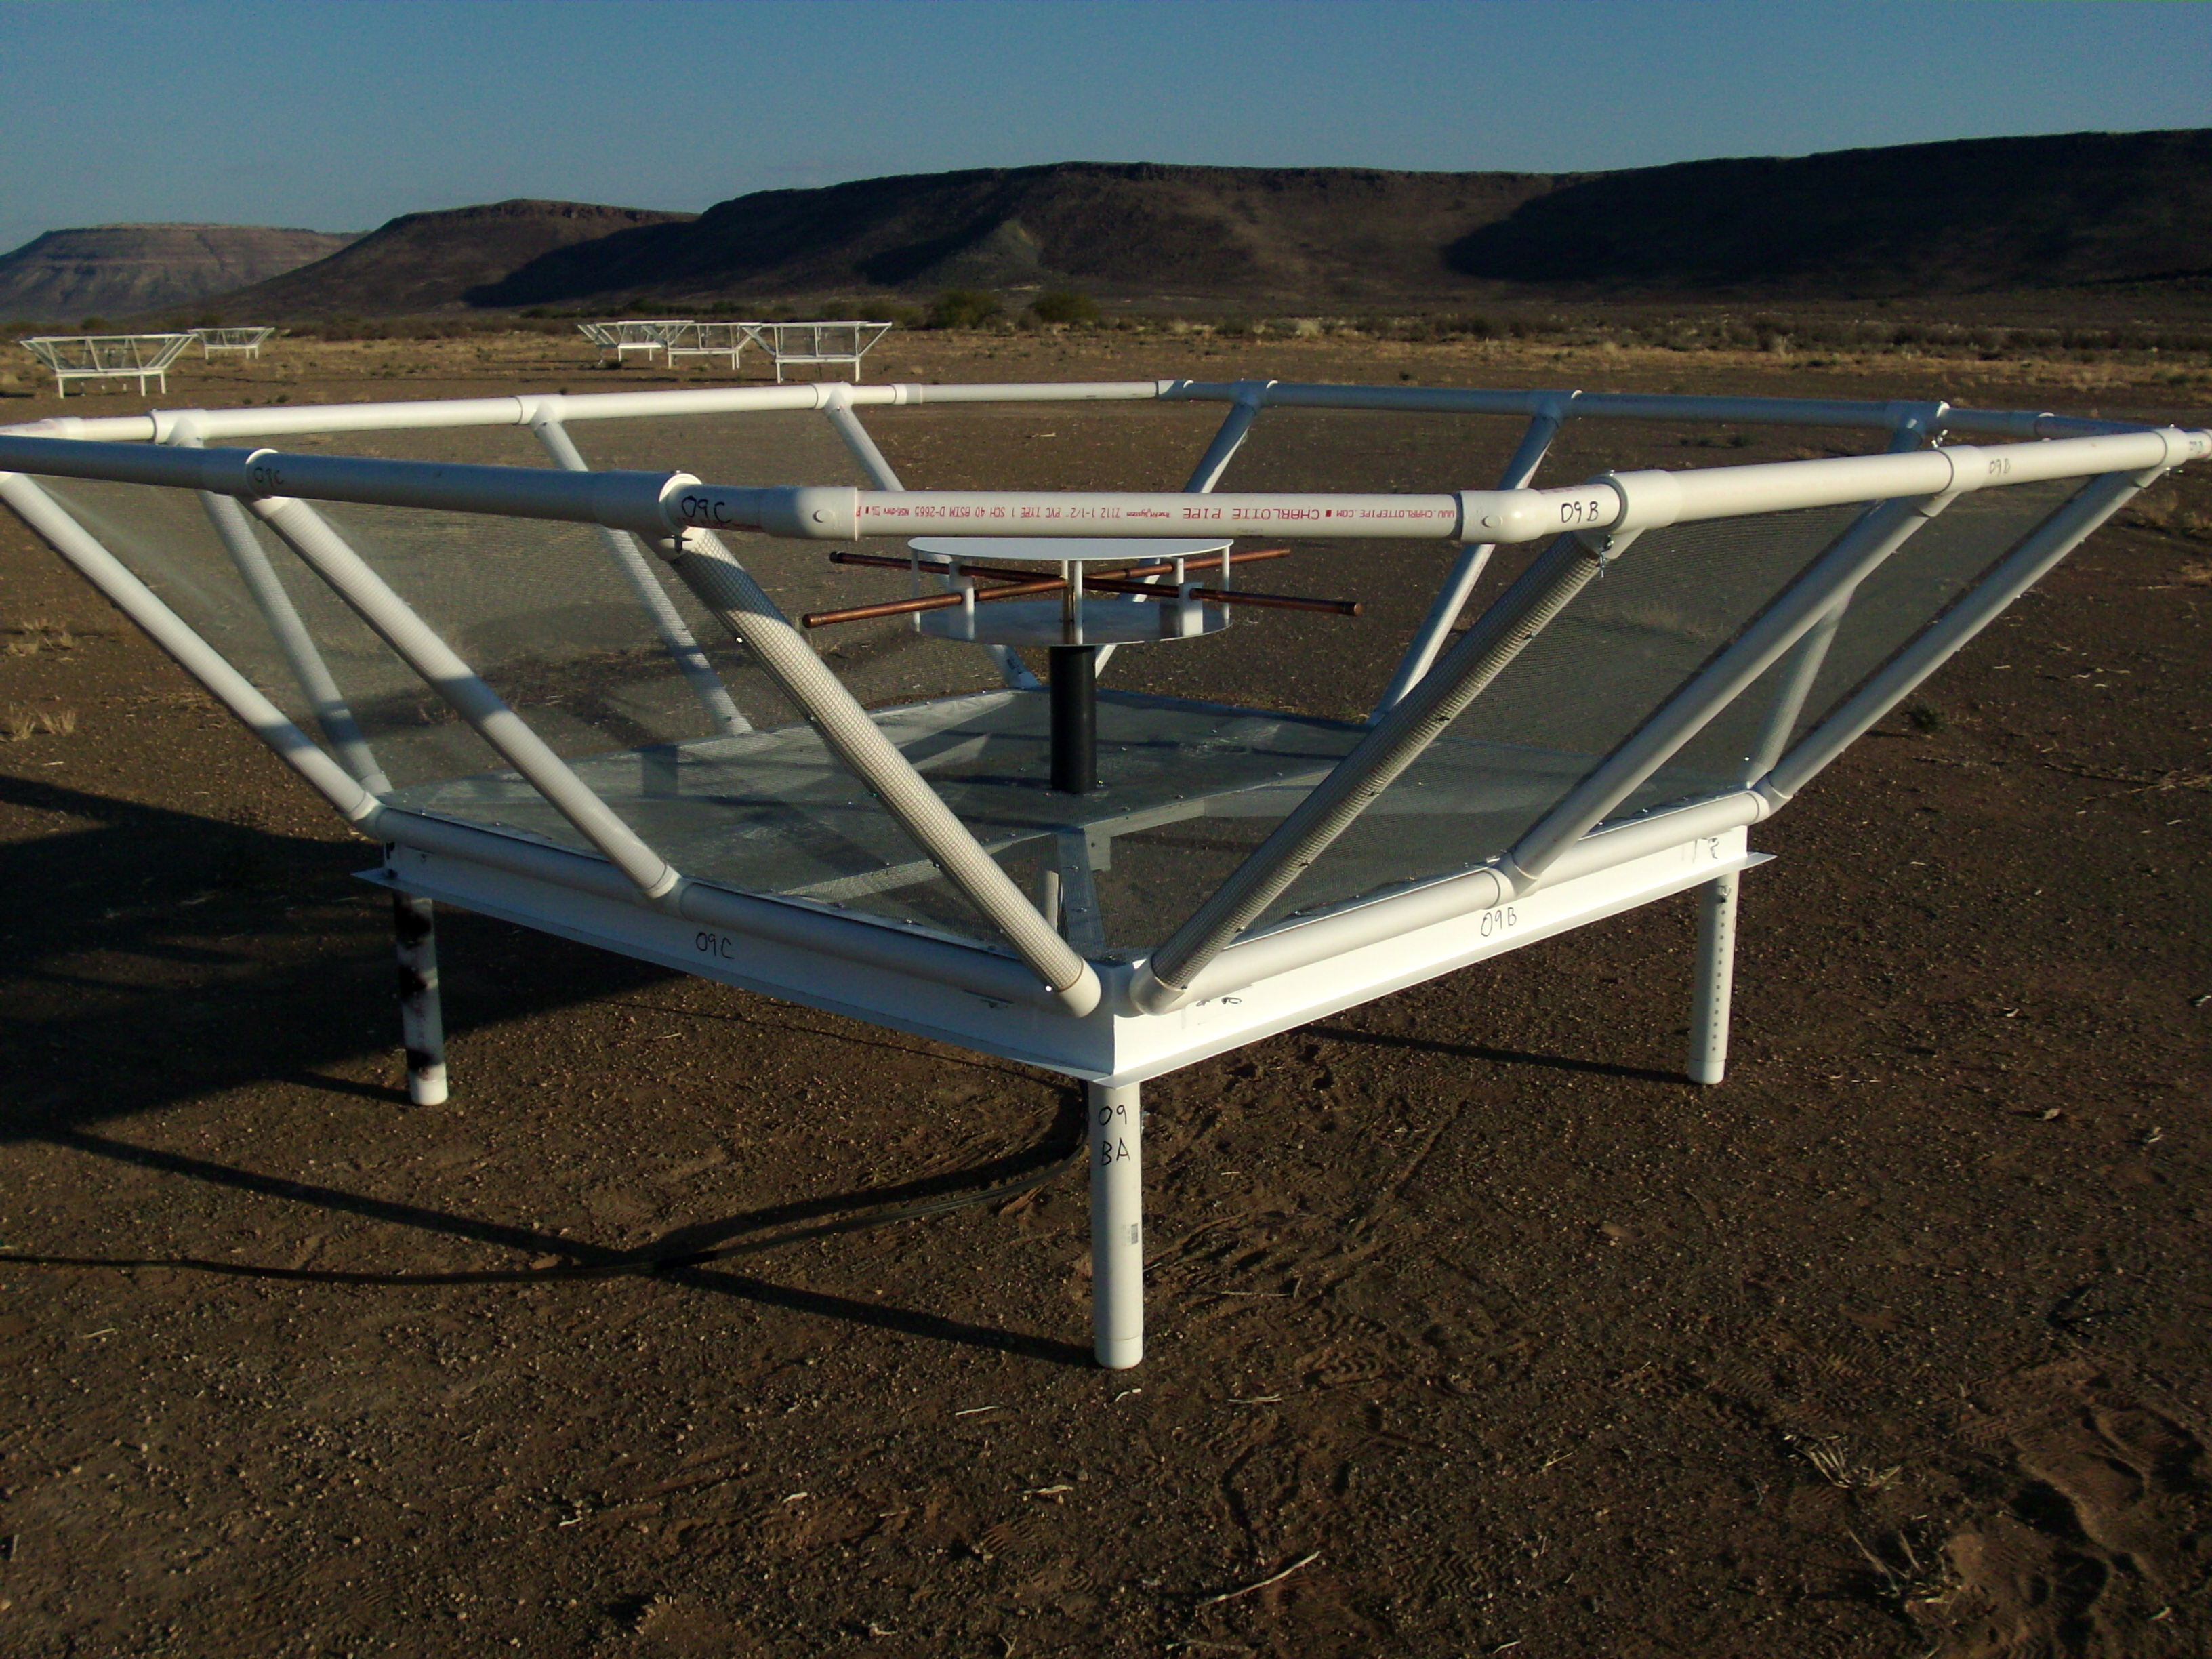
\includegraphics[height=0.35\textwidth]{plots/paper_dipole.png}
%	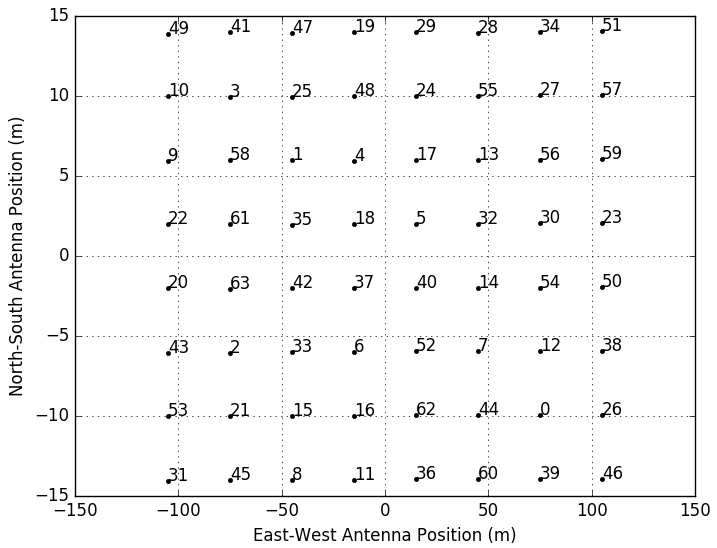
\includegraphics[height=0.35\textwidth]{plots/antenna_layout.png}
%	\caption{PAPER dipole in South Africa (left) and PAPER-64 antenna layout (right).}
%	\label{fig:paper}
%\end{figure*}

The previously best published $21$ cm upper limit result from (\citealt{ali_et_al2015}) uses $124$ nights of data to place a $2\sigma$ upper limit on $\Delta^{2}(k)$, defined as

\begin{equation}
\Delta^{\textbf{2}}\textbf{(k)} = \frac{k^{3}}{2\pi^{2}}\hat{\textbf{p}}\textbf{(k)},
\end{equation}

\noindent of $(22.4$ mK$)^{2}$ in the range $0.15 < k < 0.5$ h Mpc$^{-1}$ at $z = 8.4$. The revision of this limit stems mostly from previously underestimated signal loss and underestimated error bars \cc{cite retraction paper}, both of which we address in the case study. 

For our analysis, we use $8$ hours of LST (RA $0.5$-$8.6$ hours) and $51$ total baselines. All power spectrum results are produced using channels $95$-$115$, corresponding to a center redshift of $z=8.4$. We note that the PAPER-64 dataset that we use in this case study differs from that in \citet{ali_et_al2015} mainly by the fringe-rate filter. In \citet{ali_et_al2015}, the applied filter was degraded by widening it in fringe-rate space. This was chosen in order to increase the number of independent modes and reduce signal loss. With the development of a robust method for assessing signal loss, we feel comfortable using a narrow filter --- the optimal fringe-rate filter --- in order to maximize sensitivity. This filter is computed for a fiducial $30$ m baseline at $150$ MHz, the center frequency in our band. The filter in both the fringe-rate domain and time domain is shown in Figure \ref{fig:frp}.

\begin{figure}
	\centering
	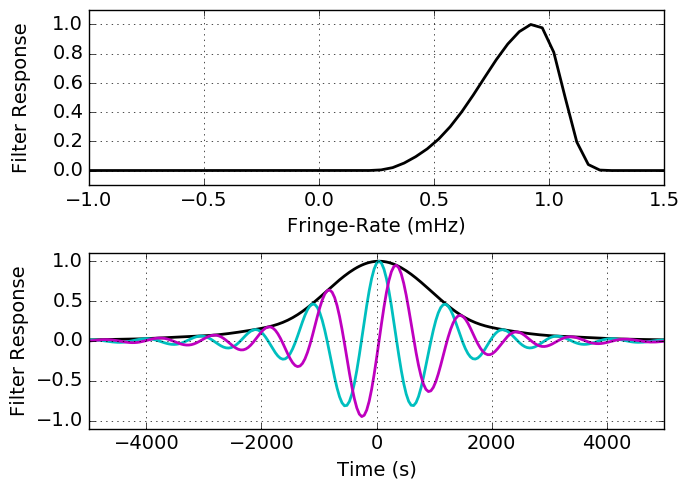
\includegraphics[width=\columnwidth]{plots/frp.png}
	\caption{Top: the normalized optimal power-spectrum sensitivity weighting in fringe-rate space for our fiducial baseline and Stokes I polarization beam. Bottom: the time-domain convolution kernel corresponding to the top panel. Real and imaginary components are illustrated in cyan and magenta, respectively, with the absolute amplitude in black. The fringe-rate filter acts as an integration in time, increasing sensitivity but reducing the number of independent samples in the dataset.}
	\label{fig:frp}
\end{figure}

\subsection{Case Study: Signal Loss}
\label{sec:Sigloss}

In Section \ref{sec:SiglossOverview}, we showed how signal loss arises when weighting data using information from itself. Here we describe a methodology that simulates the injection and recovery of a cosmological signal in order to quantify the amount of signal loss accompanying a weighting scheme. In particular, we highlight major differences from the signal loss computation used in \citet{ali_et_al2015}, which previously underestimated losses. 

\subsubsection{Signal Loss Methodology} 

We simulate an EoR signal by creating a random Gaussian signal (with a default variance of $1$) with the same shape as our data, and we fringe-rate filter this signal twice using the optimal filter. The first filter transforms the white noise into a signal that's attached to the sky (i.e. what our instrument observes). The second filter represents the fringe-rate filtering step in our data analysis pipeline. This mock EoR signal is injected on top of fringe-rate filtered PAPER-64 data at a range of amplitude levels, ranging from well-below the data level, to well-above.

Suppose that $\textbf{e}$ is the injected EoR (at some amplitude level), and $\textbf{x}$ is our data vector. We define $\textbf{r}$ to be the data plus the EoR signal:

\begin{equation}
\textbf{r} = \textbf{x} + \textbf{e}.
\end{equation}

We are interested in quantifying how much $\textbf{e}$ is lost after weighting $\textbf{r}$ and applying OQE formalism. We investigate this by comparing two quantities we define as the input power spectrum and output power spectrum: $P_{in}$ and $P_{out}$. $P_{in}$ represents the unweighted power spectrum of only $\textbf{e}$, our simulated EoR signal. $P_{out}$ is the weighted power spectrum of $\textbf{e}$ that would result from our pipeline if the signal was mixed with our data. Comparing the two quantities yields insight into how much of $\textbf{e}$ is lost due to our choice of weighting. Ignoring normalization factors, these two quantities can be written as:

\begin{equation}
P_{in,\alpha} \propto \textbf{e}^{\dagger}\textbf{I}\textbf{Q}_{\alpha}\textbf{I}\textbf{e}
\end{equation}

\noindent and

\begin{eqnarray}
\label{eq:sigloss}
P_{out,\alpha} \equiv \hat{\textbf{p}}_{e,\alpha} &=& \hat{\textbf{p}}_{r,\alpha}-\hat{\textbf{p}}_{x,\alpha} \nonumber \\
&\propto& \textbf{r}^{\dagger}\textbf{R}_{r}\textbf{Q}_{\alpha}\textbf{R}_{r}\textbf{r} - \textbf{x}^{\dagger}\textbf{R}_{x}\textbf{Q}_{\alpha}\textbf{R}_{x}\textbf{x}.
\end{eqnarray}

It is noted that the output power spectrum is comprised of two terms: the weighted power spectrum associated with \textbf{r}, and that of data \textbf{x} alone. 

One may wonder why $P_{out}$ cannot be computed simply as the weighted power spectrum of $\textbf{e}$ alone, namely $P_{out,\alpha} \propto \textbf{e}^{\dagger}\textbf{R}_{e}\textbf{Q}_{\alpha}\textbf{R}_{e}\textbf{e}$. Expanding Equation \ref{eq:sigloss}, we see that $P_{out}$ is comprised of multiple terms:

\begin{eqnarray}
\label{eq:crossterm}
P_{out,\alpha} &\propto& (\textbf{x}+\textbf{e})^{\dagger}\textbf{R}_{r}\textbf{Q}_{\alpha}\textbf{R}_{r}(\textbf{x}+\textbf{e}) - \textbf{x}^{\dagger}\textbf{R}_{x}\textbf{Q}_{\alpha}\textbf{R}_{x}\textbf{x} \nonumber \\
&\propto& \textbf{x}^{\dagger}\textbf{R}_{r}\textbf{Q}_{\alpha}\textbf{R}_{r}\textbf{x} + \textbf{e}^{\dagger}\textbf{R}_{r}\textbf{Q}_{\alpha}\textbf{R}_{r}\textbf{e} + \textbf{x}^{\dagger}\textbf{R}_{r}\textbf{Q}_{\alpha}\textbf{R}_{r}\textbf{e} \nonumber \\
&+& \textbf{e}^{\dagger}\textbf{R}_{r}\textbf{Q}_{\alpha}\textbf{R}_{r}\textbf{x} - \textbf{x}^{\dagger}\textbf{R}_{x}\textbf{Q}_{\alpha}\textbf{R}_{x}\textbf{x}.
\end{eqnarray}

Taking the case of very large $\textbf{e}$, so that $\textbf{R}_{r} \sim \textbf{R}_{e}$ and any terms involving only $\textbf{x}$ are small, yields:

\begin{eqnarray}
\label{eq:pout_expand}
P_{out, \alpha,\textbf{e} \gg \textbf{x}} &\propto& \textbf{e}^{\dagger}\textbf{R}_{e}\textbf{Q}_{\alpha}\textbf{R}_{e}\textbf{e} + \textbf{x}^{\dagger}\textbf{R}_{e}\textbf{Q}_{\alpha}\textbf{R}_{e}\textbf{e} \nonumber \\
&+& \textbf{e}^{\dagger}\textbf{R}_{e}\textbf{Q}_{\alpha}\textbf{R}_{e}\textbf{x}.
\end{eqnarray}

We see that our naive expression for $P_{out}$ is the first term in Equation \ref{eq:pout_expand}, but there are also two additional terms. An initial assumption would be that the cross-terms that involve both $\textbf{e}$ and $\textbf{x}$ should be zero, since foregrounds and the cosmological signal are physically unrelated. In \citet{ali_et_al2015}, this assumption is used, and the first term in Equation \ref{eq:pout_expand} is directly compared to the input (unweighted) power spectrum to compute signal loss.

However, deeper investigations of these terms reveal that they contain non-negligible power. In fact, foreground modes and signal modes are anti-correlated on average, as derived and explained in \citet{switzer_et_al2015}. The spurious correlation of the two means that we cannot compute signal loss using a signal-only simulation, which would yield greater values for $P_{out}$ and thereby underestimate signal loss. Therefore, in our revised signal loss computation we use the full quantity for $P_{out}$ as defined in Equation \ref{eq:sigloss}, which subtracts the weighted power spectrum of the data from the weighted power spectrum of data plus EoR. 

For the unweighted case ($\textbf{R} \equiv \textbf{I}$), we expect $P_{out}$ and $P_{in}$ to be equal, and hence the ratio $P_{in} / P_{out} = 1$. For the weighted case, this may not be true due to signal loss. To quantify the loss, we look at the ratio $P_{in}/P_{out}$ as the amplitude level of the injected signal \textbf{e} is increased. In the next section, we describe our signal loss transfer function ($P_{in}$ vs. $P_{out}$) for PAPER-64 data and detail the computation used to translate our power spectrum result into one viewed through a signal loss lens.

\subsubsection{Signal Loss in Practice}

\cc{This section needs to be filled in once our method is finalized...}

We now shift our attention towards computing signal loss for our fringe-rate filtered PAPER-64 dataset. While our methodology outlined below is robust to any weighting scheme, here we demonstrate the computation using inverse covariance weighting ($\textbf{R} = \textbf{C}^{-1}$), which leads to substantial loss. With this weighting, our expressions for $P_{in}$ and $P_{out}$ become:

\begin{eqnarray}
P_{in,\alpha} &\propto& \textbf{e}^{\dagger}\textbf{I}\textbf{Q}_{\alpha}\textbf{I}\textbf{e} \\
P_{out,\alpha} &\propto& \textbf{r}^{\dagger}\textbf{C}_{r}^{-1}\textbf{Q}_{\alpha}\textbf{C}_{r}^{-1}\textbf{r} - \textbf{x}^{\dagger}\textbf{C}_{x}^{-1}\textbf{Q}_{\alpha}\textbf{C}_{x}^{-1}\textbf{x} 
\end{eqnarray}

%\begin{figure*}
%	\centering
%	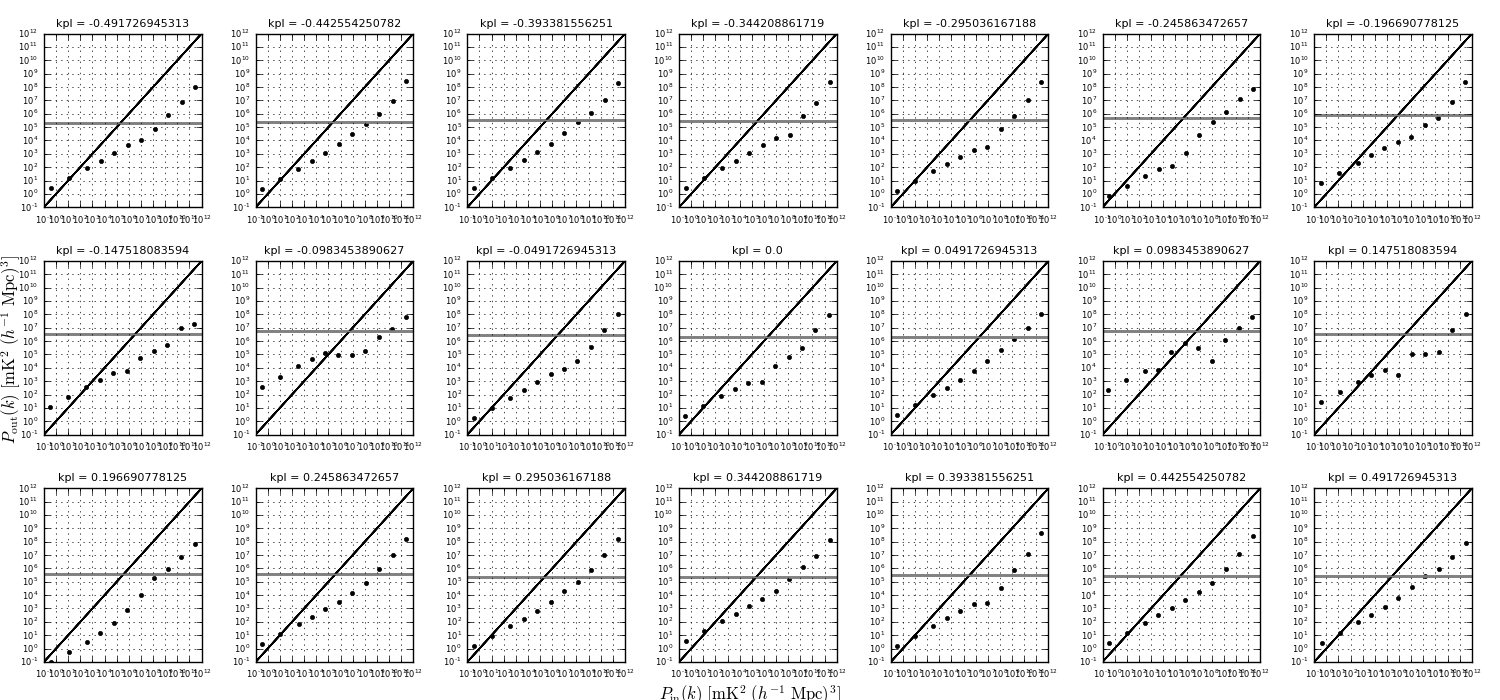
\includegraphics[width=1.0\textwidth]{plots/sigloss1_data.png}
%	\caption{$P_{in}$ vs. $P_{out}$ (black points) for 15 injection levels and 21 $k$'s. The solid grey line is the $2\sigma$ upper limit for the weighted power spectrum of PAPER-64 data, and it is at this level where the signal loss factor $P_{in}/P_{out}$ is computed by interpolation. \cc{Maybe re-do this plot with closer-together points}}
%	\label{fig:sigloss1_data}
%\end{figure*}

%\begin{figure*}
%	\centering
%	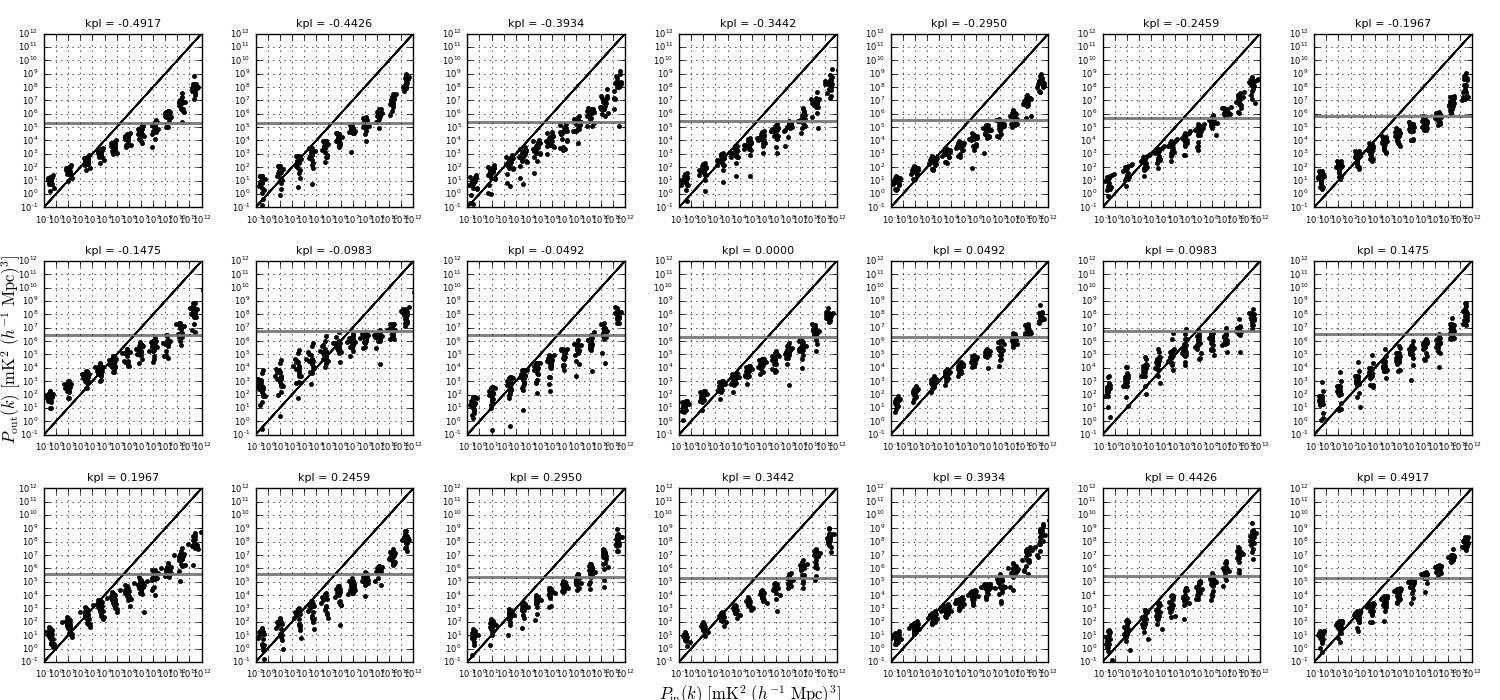
\includegraphics[width=1.0\textwidth]{plots/sigloss2_data.png}
%	\caption{$P_{in}$ vs. $P_{out}$ (black) for 15 injection levels, 20 bootstraps, and 21 $k$'s. The transparent grey region represents all PAPER-64 bootstrapped estimates.}
%	\label{fig:sigloss2_data}
%\end{figure*} 

%\begin{figure}
%	\centering
%	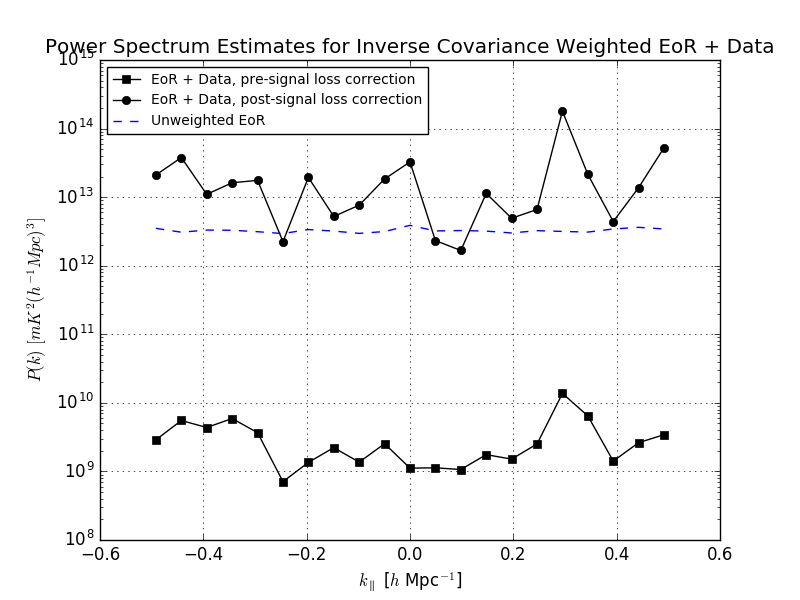
\includegraphics[width=\columnwidth]{plots/sigloss_beforeafter.png}
%	\caption{Power spectrum estimates of the combined EoR + PAPER-64 dataset, pre (squares) and post (circles) signal loss correction. The dashed blue line is the unweighted power spectrum estimate of EoR alone.}
%	\label{fig:sigloss_beforeafter}
%\end{figure}

%\begin{figure*}
%	\centering
%	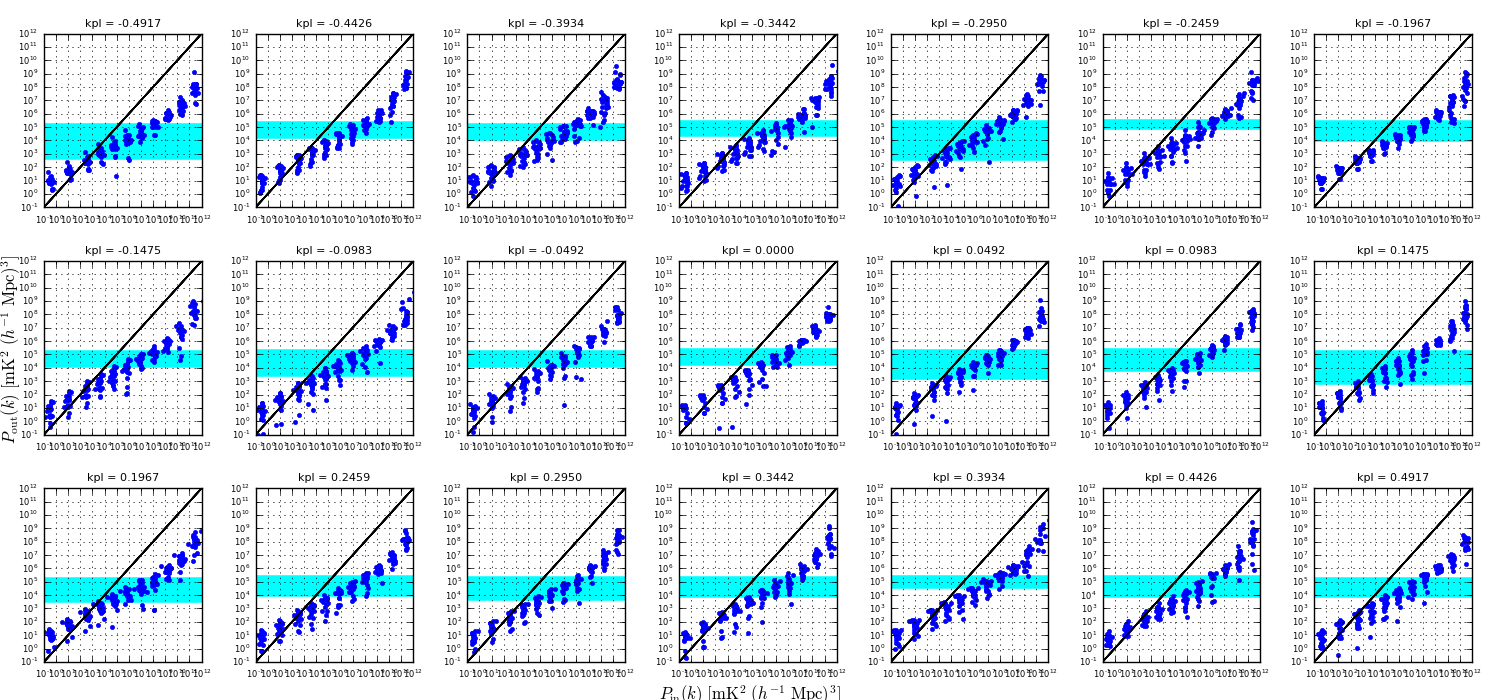
\includegraphics[width=1.0\textwidth]{plots/sigloss2_noise.png}
%	\caption{$P_{in}$ vs. $P_{out}$ (blue) for 15 injection levels, 20 bootstraps, and 21 $k$'s. \cc{Plot a semi-transparent cyan range of pCn values instead of just the max}}
%	\label{fig:sigloss2_noise}
%\end{figure*}

%\begin{figure*}
%	\centering
%	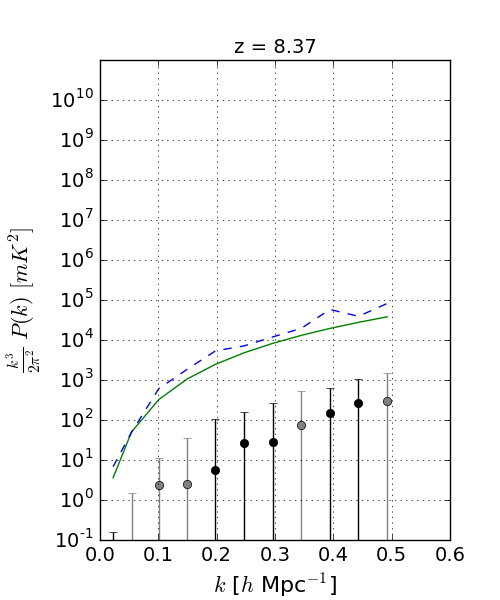
\includegraphics[width=0.4\textwidth]{plots/ps2_noise_nosigloss.png}
%	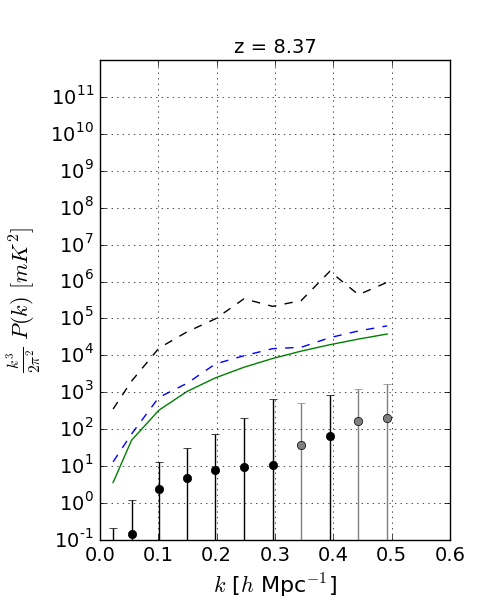
\includegraphics[width=0.4\textwidth]{plots/ps2_noise.png}
%	\caption{Full inverse covariance weighted power spectrum of pure noise (black and grey points, with $2\sigma$ error bars) before signal loss correction (left) and after (right). Black points correspond to positive values, while grey points correspond to originally negative values that have been made positive for plotting. The dashed blue line is the unweighted power spectrum ($2\sigma$ upper limit). The solid green line is the theoretical noise level prediction based on observational parameters.}
%	\label{fig:ps2_noise}
%\end{figure*}

\subsubsection{Data Weighting}
\label{sec:Weight}

\cc{This section is under construction...}

With our signal loss formalism established, we now have the capability of experimenting with different weighting options for $\textbf{R}$. Our goal here is to choose a weighting method that successfully down-weights foregrounds and systematics in our data without generating large amounts of signal loss. We have found that the balance between the two is a delicate one and requires a careful understanding and altering of covariance matrices.

Using full inverse covariance weighting, our power spectrum results before and after signal loss correction is shown in Figure \ref{fig:ps2_data}. Prior to signal loss correction, it is clear that the power spectrum is unfeasible because it is well below the theoretical noise level prediction. Post-correction, the power spectrum values blow up much higher than both the theory and unweighted power spectrum. 

%\begin{figure*}
%	\centering
%	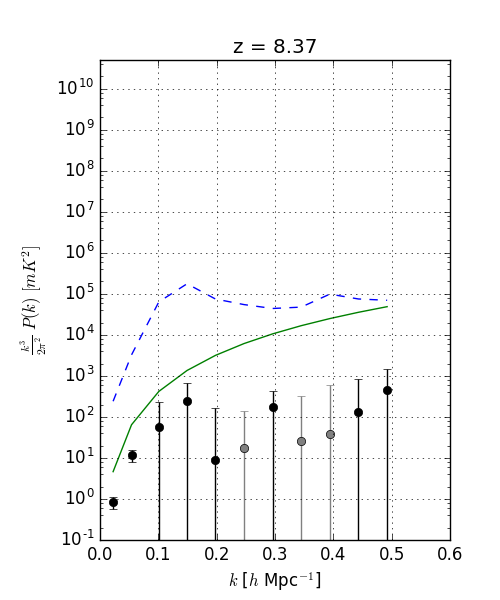
\includegraphics[width=0.4\textwidth]{plots/ps2_data_nosigloss.png}
%	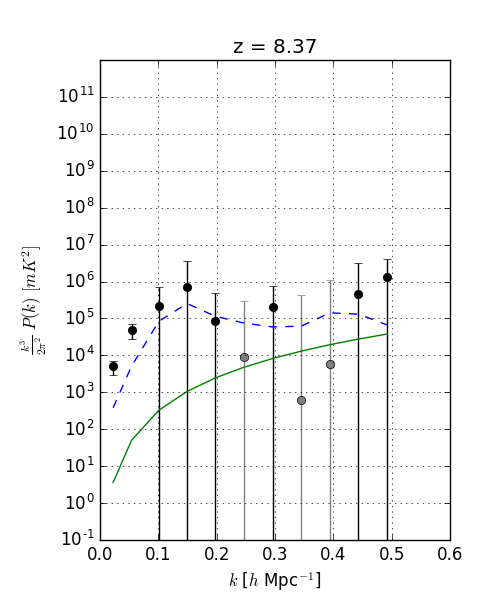
\includegraphics[width=0.4\textwidth]{plots/ps2_data.png}
%	\caption{Full inverse covariance weighted power spectrum of PAPER-64 data (black points, with $2\sigma$ error bars) before signal loss correction (left) and after (right). The dashed blue line is the unweighted power spectrum ($2\sigma$ upper limit). The solid green line is the theoretical noise level prediction based on observational parameters.}
%	\label{fig:ps2_data}
%\end{figure*}

Following our toy model investigation in Section \ref{sec:SiglossOverview}, we investigate the shape of the eigenspectrum of $\textbf{C}$ for a typical baseline used in the analysis. Figure \ref{fig:eigenspectrum} shows this spectrum for baseline (1,4). The spectrum is very steep, spanning 4 orders of magnitude, implying that different modes are given dramatically different weights. In fact, this behavior is much more extreme than we saw in the toy model, whose eigenspectrum (for the `fringe-rate filtered' case) only started to vividly steepen for the last few eigenmodes. The consequence of assigning individual weights to many more modes than are present in the data is significant --- to the point of resulting in power spectrum values that are higher than if no weighting scheme was used at all.

%\begin{figure*}
%	\centering
%	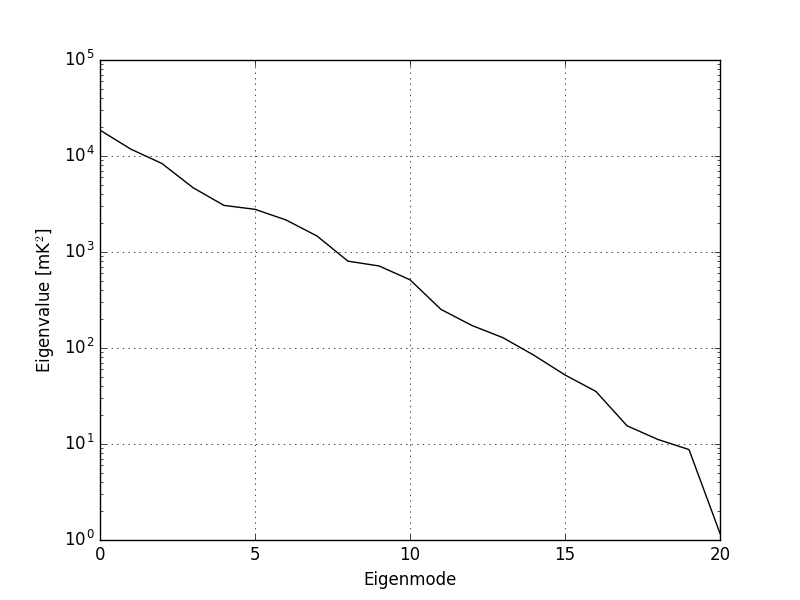
\includegraphics[width=0.4\textwidth]{plots/eigenspectrum.png}
%	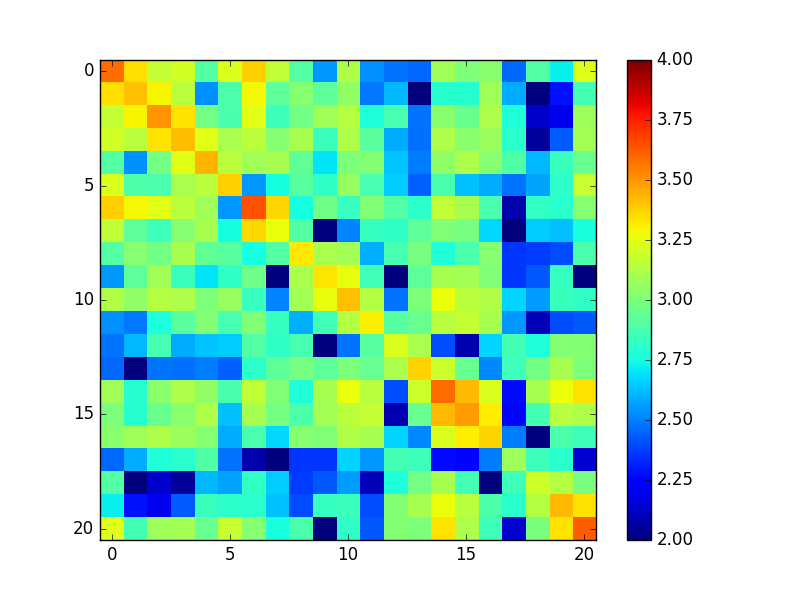
\includegraphics[width=0.4\textwidth]{plots/covariance.png}
%	\caption{Eigenspectrum for $\textbf{C}$ for baseline (1,4) for the 21 channels ofs interest (left) and covariance matrix $\textbf{C}$ for the same baseline (right).}
%	\label{fig:eigenspectrum}
%\end{figure*}

The full inverse covariance treatment of our data is suboptimal to the unweighted case, meaning that choosing such a weighting does not help suppress systematics as we intended. Now we would like to find a weighting method that does successfully down-weight contaminants in our data and make some improvement over the unweighted power spectrum. There are many choices for determining the covariance matrix $\textbf{C}$, as described in Section \ref{sec:SiglossOverview}, but here we will illustrate \cc{?} promising ones as applied to PAPER-64.

\cc{Should I just show the identity multiplication scheme that seems to be the best? Show lots of options? Mention different options but not show the results?}

\begin{figure*}
	\centering
	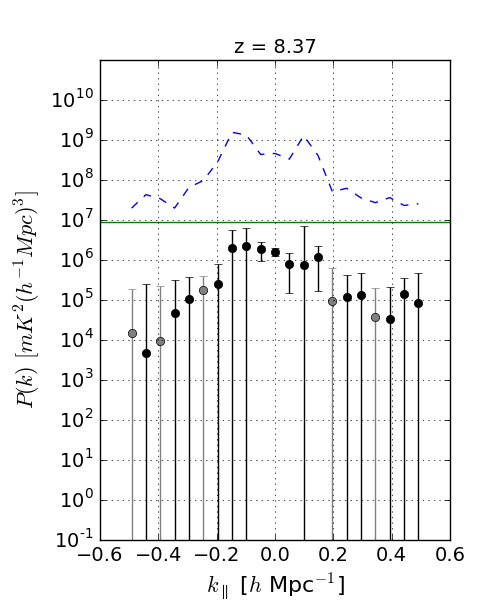
\includegraphics[width=0.4\textwidth]{plots/ps1_data_nosigloss.png}
	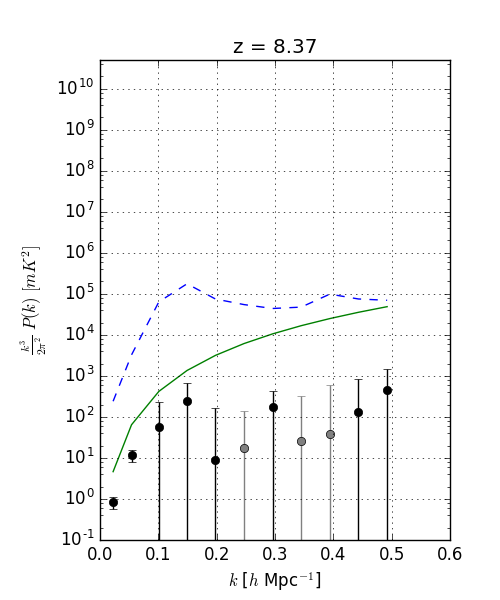
\includegraphics[width=0.4\textwidth]{plots/ps2_data_nosigloss.png}
	\caption{Highest sensitivity power spectrum of PAPER-64 using $\hat{\textbf{C}}_{eff} = \hat{\textbf{C}} * \textbf{I}$ (minimal signal loss). Black and grey points correspond to positive and negative power spectrum values, respectively, with $2\sigma$ error bars also plotted. The dashed blue line is the unweighted power spectrum ($2\sigma$ upper limit). The solid green line is the theoretical noise level prediction based on observational parameters. This power spectrum result differs from \citet{ali_et_al2015} in that it only uses data from one type of baseline ($30$ m East/West baselines) instead of three. Additionally, an optimal fringe-rate filter was used instead of a degraded one. Major differences from previously published results stem from revisions regarding signal loss, bootstrapping, and the theoretical error computation.}
	\label{fig:ps1_data}
\end{figure*}

\subsection{Case Study: Error Estimation}
\label{sec:Error}

In this section we discuss the ways in which we estimate errors for PAPER-64 power spectra. We first walk through a derivation for a theoretical error estimation based on observational parameters. Although a theoretical model often differs from true errors as explained in Section \ref{sec:ErrorOverview}, it is helpful to understand the ideal case and the factors that affect its sensitivity. We also highlight major changes in our calculation from \citet{ali_et_al2015}, which in total decrease the estimated power spectrum sensitivity of PAPER-64 by a factor of \cc{fill in when ready}. Finally, we build on the lessons learned about bootstrapping in Section \ref{sec:ErrorOverview} to revise our bootstrapping method as applied to PAPER-64 data in order to compute accurate errors from the data itself.

\subsubsection{Theoretical Error Estimation}
\label{sec:PSSense}

Theoretical errors, computed from the instrumental temperature and observational parameters, provide a useful cross-check for bootstrapped errors and is a helpful predictor of the maximum sensitivity that can be achieved by a particular observation and analysis. Here we walk through a detailed computation of a theoretical noise estimation as applied to PAPER-64 observations and highlight major changes from \citet{ali_et_al2015}. We first give a general formula, and then go into detail about each factor.

The sensitivity prediction for a power spectral analysis of interferometric $21$ cm data, in temperature-units, is:

\begin{equation}
\label{eq:sense}
p(k) = \frac{X^{2}Y \Omega_{eff} T_{sys}^{2}}{\sqrt{2N_{lsts}N_{seps}}\,t_{int}N_{days}N_{bls}N_{pols}}
\end{equation}

\begin{itemize}
\item $X^{2}Y$: Conversion factors from observing coordinates (angles on the sky) to cosmological coordinates (co-moving distances). For $z=8.4$, $X^{2}Y = 5 \times 10^{11} h^{-3} Mpc^{3} str^{-1} GHz^{-1}$.
\item $\Omega_{eff}$: The primary beam angular size. The effective beam area changes with the application of a fringe-rate filter, since parts of the beam are up-weighted and down-weighted. Using numbers from Table 1 in \citet{parsons_et_al2016}, $\Omega_{eff} = 0.74^{2}/0.24$ for an optimal fringe-rate filter. 
\item $T_{sys}$: The system temperature is set by:

\begin{equation}
\label{eq:sys}
T_{sys} = 180\Big(\frac{\nu}{0.18}\Big)^{-2.55} + T_{rcvr},
\end{equation}

where $\nu$ are frequencies in GHz. We use a receiver temperature of $200$ K, yielding $T_{sys} = 487$ at $150$ MHz. This is lower than in \citet{ali_et_al2015} because \cc{why?}.
\item $\sqrt{2}$: This factor in the denominator of the sensitivity equation comes from only using the real part of power spectrum estimates when plotting and quoting upper limits (imaginary component is discarded).
\item $N_{lsts}$: The number of LST hours that go into a power spectrum estimation. The sensitivity scales as the square root because we integrate incoherently over time. For PAPER-64, $N_{lsts} = 8$ hours.
\item $N_{seps}$: The number of baseline separation types averaged incoherently in a final power spectrum estimate. For the analysis in this paper, we only use one type of baseline, hence $N_{seps}=1$.
\item $t_{int}$: The integration time of the data. It is crucial to adapt this number if filtering is applied along the time axis (i.e. a fringe-rate filter). We compute the effective integration time of our fringe-rate filtered data by scaling the original integration time using the following:
\begin{equation}
t_{frf} = t_{int} \frac{\int1 \, df}{\int w^{2}(f) \,df},
\end{equation}
where $t_{int}=43$ seconds, $t_{frf}$ is the fringe-rate filtered integration time, $w$ is the fringe-rate profile, and the integral is taken over all fringe-rates. In other words, we calculate the effective integration time by computing how our beam is altered in fringe-rate space. For PAPER-64, this number is $t_{int} = 3857$ s. 
\item $N_{days}$: The total number of days of data analyzed. In \citet{ali_et_al2015}, this number was set to $135$. However, because we divide our data in half (to form `even' and `odd' datasets), this number should be reduced by a factor of $2$. Additionally, because our $LST$ coverage is not $100\%$ complete (it doesn't overlap for every single day), we compute a realistic value of $N_{days}$ as the RMS of all the daily counts in one dataset (`even', for example). For PAPER-64, our revised estimate of $N_{days}$ is $\sim34$ days.
\item $N_{bls}$: The number of baselines contributing to the sensitivity of a power spectrum estimate. In \citet{ali_et_al2015}, this number was the total number of $30$ m East/West baselines used in the analysis. However, using the total number of baselines neglects the fact that we divid baselines into $5$ groups before cross-multiplying data. Our revised estimate for the parameter is $N_{bls} = \frac{N_{bls}}{N_{gps}}\sqrt{N_{gps}^{2}-N_{gps}}$, where $N_{gps} = 5$. This expression arises because $N_{bls}$ must be scaled by the total number of cross-multiplications going into the power spectrum estimate. For $5$ groups, there are $25$ total cross-products, minus $5$ cross-products since we avoid multiplying the same group with itself. For our PAPER-64 analysis with only one baseline separation type, this becomes $N_{bls} \sim 46$ baselines. 
\item $N_{pols}$: The number of polarizations averaged together. For the case of Stokes I, $N_{pols}=2$.
\end{itemize}

Equation \ref{eq:sense} represents the most sensitive estimate for $\hat{\textbf{p}}(k)$ given our observing parameters. An additional factor of $\sqrt{2}$ is gained in sensitivity when folding our power spectra into $\Delta^{2}(k)$, due to averaging together positive and negative $k$'s. 

To verify our thermal noise prediction, we form power spectra estimates using a pure noise simulation. We create Gaussian random noise and use $T_{sys}$ in order to best represent the thermal noise level of PAPER-64 data. We convert $T_{sys}$ into a variance statistic using:

\begin{equation}
T_{rms} = \frac{T_{sys}}{\sqrt{\Delta\nu \Delta t N_{days} N_{pols}}},
\end{equation}

where $\Delta\nu$ is channel spacing, $\Delta t$ is integration time, $N_{days}$ is the number of daily counts for a particular time and frequency that went into our LST binned set, and $N_{pols}$ is the number of polarizations ($2$ for Stokes I). This rms temperature sets the variance of the Gaussian random noise.

We fringe-rate filter the noise in the same way as PAPER-64 data, using an optimal fringe-rate filter. Power spectrum results for the noise simulation are shown in Figure \ref{fig:ps_noise}, where the black and grey points represent positive and negative power spectrum values, respectively (with $2\sigma$ error bars and $\hat{\textbf{C}} = \hat{\textbf{C}} * \textbf{I}$), the dashed blue line represents the unweighted power spectrum, and the solid green line denotes our $2\sigma$ theoretical noise prediction as calculated by Equation \ref{eq:sense}. All three are in agreement, validating our analytical thermal noise calculation. 

\begin{figure*}
	\centering
	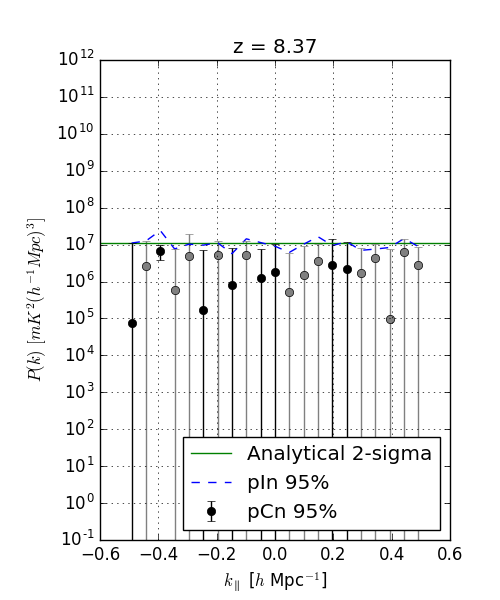
\includegraphics[width=0.4\textwidth]{plots/ps_noise_pk.png}
	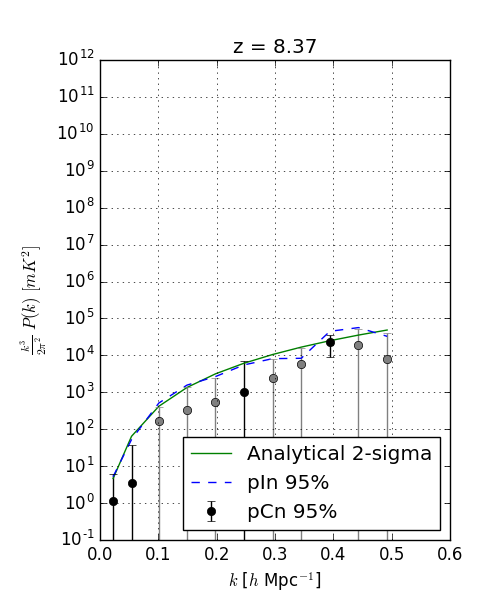
\includegraphics[width=0.4\textwidth]{plots/ps_noise_delta.png}
	\caption{Power spectrum estimate for a noise simulation that mimics the noise level of PAPER-64 data. The weighted power spectrum points and $2\sigma$ errors are show in black and grey (positive and negative values), where we regularize $\hat{\textbf{C}}$ by setting $\hat{\textbf{C}} = \hat{\textbf{C}} * \textbf{I}$ to minimize signal loss. The dashed blue line is the unweighted power spectrum (also $2\sigma$ upper limit). The solid green line is the theoretical noise level prediction as calculated by Equation \ref{eq:sense}. All three estimates agree.}
	\label{fig:ps_noise}
\end{figure*}

\subsubsection{Bootstrapping}
\label{sec:Boot}

We bootstrap PAPER-64 power spectra in order to determine confidence intervals for our results. In this section, we highlight two major changes in the way we estimate errors since \citet{ali_et_al2015}, using the lessons we've learned about sampling with replacement and bootstrapping independent samples.

As discussed in Section \ref{sec:ErrorOverview}, bootstrapping is only a valid way of estimating errors if a dataset is comprised of independent samples. The PAPER-64 pipeline outputs $N$ bootstraps (over baselines), each a $2$-dimensional power spectrum that is a function of $k$ and time. In \citet{ali_et_al2015}, a second round of bootstrapping occurs over the baseline bootstrap and time axes simultaneously. Random values are sampled with replacement along both axes, drawing as many values as there are number of bootstraps and times. Final power spectrum limits are then computed by taking the mean and standard deviation over this second bootstrap axis (which is typically large, on the order of $N_{boot} \sim 400$). 

Because our dataset is fringe-rate filtered, we have substantially increased our integration time, resulting in fewer independent samples (from $\sim700$ samples to $8$ samples). A random draw of $700$ samples from this dataset therefore has many repeated samples, and the variance between hundreds ($N_{boot}$) of these random samples is smaller than the true underlying variance of the data. Another way of describing this underestimation is that there are fewer ways to randomly sample data with $8$ independent modes versus $700$, so bootstrapping a fringe-rate filtered dataset yields a narrower distribution of values from which we calculate its standard deviation.

To prevent error underestimation, we simply take the average along the time axis in our revised pipeline rather than bootstrapping. Hence, our final power spectrum errors are calculated from the standard deviation over the baseline bootstrapping axis only, which is still a valid axis since each baseline makes an independent measurement of the sky.

The second aspect of bootstrapping discussed in Section \ref{sec:ErrorOverview} is the overestimation of errors which arises from repeated values in a randomly sampled bootstrap. In order to maximize sensitivity, we have revised the method by which we sample baselines when bootstrapping to ensure mostly independent samples.

First, we speed things up in our pipeline by separating our total number of baselines into $5$ groups (yielding $10$ baselines per group), where there are no repeated baselines within or between groups. In \citet{ali_et_al2015}, each group is then sampled with replacement to create a new group of the same size, which can have repeated baselines inside it. In doing so, we are sacrificing some of our sensitivity since there ends up being $3$-$4$ repeated baselines per group (Figure \ref{fig:toy_error2} shows a fraction of independent samples of $\sim55\%$ for $10$ total independent samples) . In order to maximize our sensitivity but still apply random sampling for use in error estimation, we instead form new groups using all independent baselines except the very last one, which we fill randomly. We use this method for every bootstrap, creating new groups and sampling the last spot randomly each time.

Power spectrum estimates for PAPER-64 fringe-rate filtered data are shown in Figure \ref{fig:data_errors}. The estimates use a weighting matrix of $\textbf{C}_{eff}^{-1}$, where $\textbf{C}_{eff} = \hat{\textbf{C}}*\textbf{I}$, in order to minimize signal loss. We show upper limits ($2\sigma$ error bars) for three different results. Our revised error estimation method is in black, where we only bootstrap along the baseline axis and we maximize sensitivity by random sampling only the last baseline in each group. The red curve uses a similar method except all baselines are randomly sampled, leading to a higher power spectrum estimate because some baselines are repeated per group. In blue, we bootstrap along both the baseline and time axes, drawing as many samples as there are in the data. We under-estimate errors in doing so because we are drawing many more samples than independent ones.

\begin{figure}
	\centering
	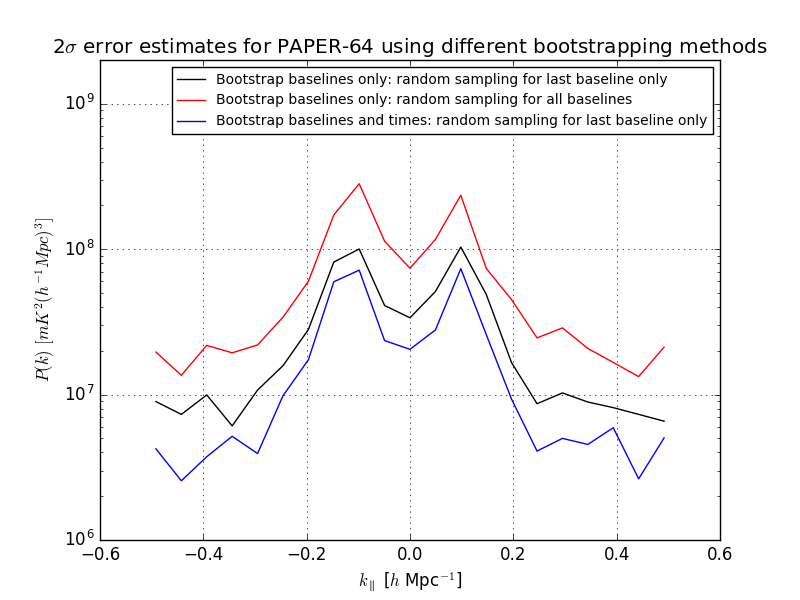
\includegraphics[width=\columnwidth]{plots/data_errors.png}
	\caption{$2\sigma$ upper limit power spectrum estimates using PAPER-64 data and three different bootstrapping methods. The data is fringe-rate filtered and a weighting matrix of $\textbf{C}_{eff}^{-1}$ is used, where $\hat{\textbf{C}}_{eff} = \textbf{C}*\textbf{I}$, in order to minimize signal loss. Three different bootstrapping methods are shown: the black and red use methods where bootstrapping occurs on the baseline axis only (not the time axis), and they differ by how the baselines are randomly sampled. It is evident that sensitivity is maximized when baselines are sampled in a way that ensures mostly independent samples (only the last baseline spot is sampled randomly). The blue result bootstraps over both the baseline and time axes, and illustrates how errors can be under-estimated if sampling more values than independent ones (fringe-rate filtering reduces the number of independent samples).}
	\label{fig:data_errors}
\end{figure}

\subsection{Case Study: Bias}
\label{sec:Bias}

In Section \ref{sec:BiasOverview} we highlighted some common sources of bias that can show up as a power spectrum detection and imitate EoR. We discussed the importance of using jackknife and null tests for instilling confidence in an EoR detection, as well as identifying other sources of biases. Here we demonstrate methods used by PAPER-64 to mitigate foreground and noise bias and we perform jackknife and null tests in order to characterize the stability and implications of our results.

\subsubsection{Mitigating Bias}

We briefly discuss one way in which we mitigate foreground leakage in a power spectrum estimate, and two in which we suppress noise biases. These methods are not novel to this analysis but here we frame them in the context of minimizing false (non-EoR) detections.

Tailoring window functions is one way to suppress foreground biases. As alluded to in Section \ref{sec:SiglossOverview}, we have a choice for the normalization matrix $\textbf{M}$ in Equation \ref{eq:phat}. For the analysis of PAPER-64 data, we compute $\textbf{M}$ using the Fisher matrix $\textbf{F}$, defined as:

\begin{equation}
\textbf{F}_{\alpha\beta} = \frac{1}{2} \text{tr} [\textbf{R}\textbf{Q}_{\alpha}\textbf{R}\textbf{Q}_{\beta} ]
\end{equation}

\noindent where $\textbf{R}$ is the data-weighting matrix and $\alpha$ and $\beta$ are wavebands in $k_{\parallel}$. We take the Cholesky decomposition of $\textbf{F}$, decomposing it into two lower triangular matrices:

\begin{equation}
\textbf{F} = \textbf{LL}^{\dagger}.
\end{equation}

\noindent Next, we construct $\textbf{M}$:

\begin{equation}
\textbf{M} = \textbf{DL}^{-1}
\end{equation}

\noindent where $\textbf{D}$ is a diagonal matrix. In doing so, our window function, defined as $\textbf{W} = \textbf{MF}$, becomes:

\begin{equation}
\textbf{W} = \textbf{DL}^{\dagger}.
\end{equation}

\noindent Because of the nature of the lower triangular matrix, this window function has the property of preventing the leakage of foreground power from low $k$ to high $k$ modes. Specifically, we order the elements in $\textbf{F}$ in such a way so that power can leak from high $k$ modes to low $k$ modes, but not vice versa. Since most foreground power shows up at low $k$'s, this method ensures a window function that retains clean, noise-dominated measurements while minimizing the contamination of foreground bias.

In addition to mitigating foreground bias at high $k$'s, two other sources of bias that we actively suppress in the PAPER-64 analysis are noise bias associated with the squaring of thermal noise and noise bias from crosstalk. In order to avoid the former, we filter out certain cross-multiplications when forming $\hat{q}$ in Equation \ref{eq:qhat}. Namely, the PAPER-64 dataset is divided into two halves: even julian dates and odd julian dates. Our data vectors are then $\textbf{x}_{even, 1}$ for the `even' dataset and baseline group $1$, $\textbf{x}_{odd, 1}$ for the `odd' dataset and baseline group $1$, etc. We only form $\hat{q}$ when the two copies of $\textbf{x}$ come from different groups and baselines, never multiplying `even' with `'even', for example, in order to prevent the squaring of the same thermal noise.

To mitigate crosstalk bias, which appears as a static bias in time, we apply a fringe-rate filter that suppresses fringe-rates of zero. Figure \ref{fig:frp} shows that the filter response is zero for such static signals. The effect of filtering out zero fringe-rates on power spectrum results is shown in \citet{ali_et_al2015}. Most notably, power spectrum detections exist at all $k$'s without crosstalk removal and these are detections that, depending on the power spectrum level, could be mistaken for EoR. 

\subsubsection{Jack-Knife Tests}

The highest sensitivity power spectrum results using PAPER-64 data, shown in Figure \ref{fig:ps1_data}, have positive biases. As discussed in Section \ref{sec:BiasTypes}, the detections that appear at low $k$ values are most likely attributable to foreground leakage. However, the positive biases at higher $k$ values require further investigation. 


\cc{Describe some jackknife tests done on PAPER-64 data, such as random signs to baselines and even/odd summing and differencing} \\
\cc{Need to explain positive bias still... not sure where it comes from yet!}

\section{Conclusion}
\label{sec:Con}

\section{Acknowledgements}
\cc{NSF Graduate Research Fellowship Program (GRFP) Fellowship}
\cc{UC Berkeley Chancellor's Fellowship}
\label{sec:Ack}

\appendix
\section{A toy model for signal loss}
\label{sec:sigloss_appendix}

In this Appendix, we examine a toy model for signal loss. Our goal is to build intuition by deriving an analytic formula for power spectrum signal loss. We will also show that in general, signal loss appears as a multiplicative bias on one's power spectrum estimate.

The minimum-variance quadratic estimator $\hat{p}_\alpha$ for the $\alpha$th bandpower of the power spectrum is given by \acl{We need to decide whether the Q matrices have their Greek indices as upper or lower indices.} \acl{Also need to state in a footnote that for this section only we'll assume without loss of generality that the data are real}
\begin{equation}
\hat{p}_\alpha = \frac{1} {2 \F_{\alpha \alpha} }\x^t \C^{-1} \Q^{\alpha} \C^{-1} \x,
\end{equation}
where
\begin{equation}
F_{\alpha \alpha} \equiv \frac{1}{2} \textrm{tr} \left( \C^{-1} \Q^\alpha \C^{-1} \Q^\alpha \right)
\end{equation}
is the $\alpha$th diagonal element of the Fisher matrix. In our case, however, we do not have \emph{a priori} knowledge of the covariance matrix. Thus, we replace $\C$ with $\Chat$, its data-derived approximation. Our estimator then becomes
\begin{equation}
\label{eq:phatloss}
\hat{p}_\alpha^\textrm{loss} = \frac{1} {2 \F_{\alpha \alpha} }\x^t \Chat^{-1} \Q^{\alpha} \Chat^{-1} \x,
\end{equation}
where
\begin{equation}
\hat{F}_{\alpha \alpha} \equiv \frac{1}{2} \textrm{tr} \left( \Chat^{-1} \Q^\alpha \Chat^{-1} \Q^\alpha \right),
\end{equation}
with the label ``loss" to foreshadow the fact that this will be an estimator with signal loss (i.e., a multiplicative bias of less than unity). We will now provide an explicit demonstration of this by modeling the estimated covariance as
\begin{equation}
\label{eq:ChatDef}
\Chat = (1-\eta) \C + \eta \x \x^t,
\end{equation}
where $\eta$ is parameter quantifying our success at estimating the true covariance matrix. If $\eta = 0$, our covariance estimate has perfectly modeled the true covariance and $\Chat = \C$. On the other hand, if $\eta =1$, then our covariance estimate is based purely on the one realization of the covariance that is our actual data, and we would expect a high level of overfitting and signal loss.

Our strategy for computing the signal loss will be to insert Eq. \eqref{eq:ChatDef} \acl{Make sure we're consistent w.r.t. ``Equation" vs. ``Eq."} into Eq. \eqref{eq:phatloss} and to express the resulting estimator $\hat{p}_\alpha^\textrm{loss}$ in terms of $\hat{p}_\alpha$. We begin by expressing $\Chat^{-1}$ in terms of $\C^{-1}$ using the Woodbury identity so that
\begin{equation}
\Chat^{-1} = \frac{\C^{-1}}{1-\eta} \left[ \I - \frac{\eta \x \x^t \C^{-1}}{1+ \eta (g-1)}\right],
\end{equation}
where we have defined $g \equiv \x^t \C^{-1} \x$. Inserting this into our Fisher estimate we have
\begin{equation}
\hat{F}_{\alpha \alpha} = \frac{F_{\alpha \alpha}}{(1-\eta)^2} \left[ 1 -\frac{\eta }{1+ \eta (g-1)} \frac{h_{\alpha \alpha}}{F_{\alpha \alpha}} + \frac{1}{2} \left( \frac{\eta }{1+ \eta (g-1)} \right)^2 \frac{h_\alpha^2}{F_{\alpha \alpha}}\right],
\end{equation}
where $h_\alpha \equiv \x^t \C^{-1} \Q^\alpha \C^{-1} \x $ and $h_{\alpha \alpha} \equiv \x^t \C^{-1} \Q^\alpha \C^{-1} \Q^\alpha \C^{-1}\x $. Note that $g$, $h_\alpha$, and $h_{\alpha \alpha}$ are all random variables, since they depend on $\x$. Inserting these expressions into our estimator gives
\begin{eqnarray}
\label{eq:phatlossexpanded}
\hat{p}_\alpha^\textrm{loss} &=& \frac{1}{2} \frac{h_\alpha}{F_{\alpha \alpha}} \left[ 1 - \frac{\eta g}{1+ \eta (g-1)}\right]^2  \left[ 1 -\frac{\eta }{1+ \eta (g-1)} \frac{h_{\alpha \alpha}}{F_{\alpha \alpha}} + \frac{1}{2} \left( \frac{\eta }{1+ \eta (g-1)} \right)^2 \frac{h_\alpha^2}{F_{\alpha \alpha}}\right]^{-1} \nonumber \\
&=& \frac{1}{2} \frac{h_\alpha}{F_{\alpha \alpha}}\left(1-2\beta + \beta^2\right)\sum_{n=0}^\infty \sum_{k=0}^n {n \choose k} \left( \frac{\varepsilon h_{\alpha \alpha}}{F_{\alpha \alpha}}\right)^k \left( - \frac{\varepsilon^2 h_\alpha^2}{2 F_{\alpha \alpha}}\right)^{n-k},
\end{eqnarray}
where $\beta \equiv \eta g/[1+ \eta (g-1)]$ and $\varepsilon \equiv \beta / g$. To proceed, we take the ensemble average of $\hat{p}_\alpha^\textrm{loss}$ to understand its average statistical properties. Inspecting Eq. \eqref{eq:phatlossexpanded}, we see that its expectation value is a linear sum of terms of the form $\langle \beta^a h_\alpha^b h_{\alpha \alpha}^c \rangle$, where $a$, $b$, and $c$ are integers. Expanding $\beta$ in powers of $g$, we have
\begin{equation}
\label{eq:betahh}
\langle \beta^a h_\alpha^b h_{\alpha \alpha}^c \varepsilon^d \rangle = \sum_{m_1 = 1}^\infty \cdots \sum_{m_{a+d} = 1}^\infty \frac{(-\eta)^{m_1 + \dots + m_{a+d}}}{(1-\eta)^{m_1 + \dots + m_a}} \langle g^{m_1 + \dots + m_{a+d}-d} h_\alpha^b h_{\alpha \alpha}^c \rangle.
\end{equation}
Writing out the ensemble averaged quantity on the right hand side and defining $M \equiv m_1 + \dots + m_{a+d}$ yields
\begin{eqnarray}
\langle g^{m_1 + \dots + m_{a+d}} h_\alpha^b h_{\alpha \alpha}^c \rangle &=& \langle (\x^t \C^{-1} \x)^M (\x^t \C^{-1} \Q^\alpha \C^{-1} \x)^b (\x^t \C^{-1} \Q^\alpha \C^{-1} \Q^\alpha \C^{-1}\x )^c \rangle \nonumber \\
&=& \sum_{i_1}^N \sum_{j_1}^N \cdots  \sum_{k_1}^N \sum_{l_1}^N \cdots  \sum_{p_1}^N \sum_{q_1}^N \cdots  ( \C^{-1} \Q^\alpha \C^{-1} \Q^\alpha \C^{-1} )_{p_1 q_1} \dots (\C^{-1} \Q^\alpha \C^{-1} \Q^\alpha \C^{-1})_{p_c q_c}  \nonumber \\
&&  \times ( \C^{-1} \Q^\alpha \C^{-1})_{k_1 l_1} \dots ( \C^{-1} \Q^\alpha \C^{-1})_{k_b l_b} \C^{-1}_{i_1 j_1}\dots \C^{-1}_{i_M j_M} \langle x_{i_1} x_{j_1} \dots   x_{k_1} x_{l_1} \dots  x_{p_1} x_{q_1} \dots \rangle, \quad
\end{eqnarray}
where $N$ is the length of vector $\x$, i.e., the number of data points. To further simplify this expression, we assume that the data are Gaussian distributed. The expectation value on the right hand side can then be reduced to a sum of product of covariances, where each term in the sum is comprised of a particular way to partition the copies of $x$ into pairs. However, in the limit of large $N$ one particular partitioning dominates, and the result can be approximated as \acl{Should probably explain this more fully}
\begin{equation}
\langle g^{m_1 + \dots + m_{a+d}} h_\alpha^b h_{\alpha \alpha}^c \rangle \approx N^{m_1 + \dots + m_{a+d}} \left[ \textrm{tr} (\C^{-1} \Q^\alpha )\right]^b (2 F_{\alpha \alpha})^c,
\end{equation}
and re-inserting this into Eq. \eqref{eq:betahh} yields
\begin{equation}
\langle \beta^a h_\alpha^b h_{\alpha \alpha}^c \varepsilon^d \rangle \approx \left[ \frac{\eta N}{1+\eta (N-1)} \right]^a \left[ \frac{\eta }{1+\eta (N-1)} \right]^d \left[ \textrm{tr} (\C^{-1} \Q^\alpha )\right]^b (2 F_{\alpha \alpha})^c.
\end{equation}
With this result, taking the ensemble average of Eq. \eqref{eq:phatlossexpanded} is relatively straightforward. One simply replaces every copy of $\beta$ with $\beta_N \equiv \eta N / [1 + \eta (N-1)]$, every copy of $\varepsilon$ with $\varepsilon_N \equiv  \eta  / [1 + \eta (N-1)]$, every copy of $h_\alpha$ with $ \textrm{tr} (\C^{-1} \Q^\alpha )$, and every copy of $h_{\alpha \alpha}$ with $2F_{\alpha \alpha}$. Performing these substitutions and recalling \acl{make sure the reader will indeed be recalling at this point} that $\langle \hat{p}_\alpha \rangle = \langle h_\alpha \rangle / 2 F_{\alpha \alpha}$, we obtain
\begin{equation}
\frac{\langle \hat{p}_\alpha \rangle}{\langle \hat{p}_\alpha^\textrm{loss} \rangle} = \frac{1- 2\varepsilon_N + \varepsilon_N^2 \left[ \textrm{tr} (\C^{-1} \Q^\alpha) \right]^2 / 2F_{\alpha \alpha}}{(1-\beta_N)^2}.
\end{equation}
This quantity is in general less than unity, and quantifies the signal loss relative to the ideal estimator $\hat{p}_\alpha$ where we know the true covariance $\C$. As an illustrative example, for cases where $\C \propto \I$, this reduces to
\begin{equation}
\frac{\langle \hat{p}_\alpha \rangle}{\langle \hat{p}_\alpha^\textrm{loss} \rangle}  \Bigg{|}_{\C \propto \I} = \left( \frac{1-\varepsilon_N}{1-\beta_N} \right)^2 = \left[\frac{1+ \eta(N-2)}{1- \eta}\right]^2.
\end{equation}
This is shown in Figure \ref{fig:analytic_sig_loss} for $N=20$. As expected, the signal loss factor is unity for $\eta=0$ (perfect estimation of $\C$) and goes to infinity as $\eta$ approaches $1$.
\begin{figure}
	\centering
	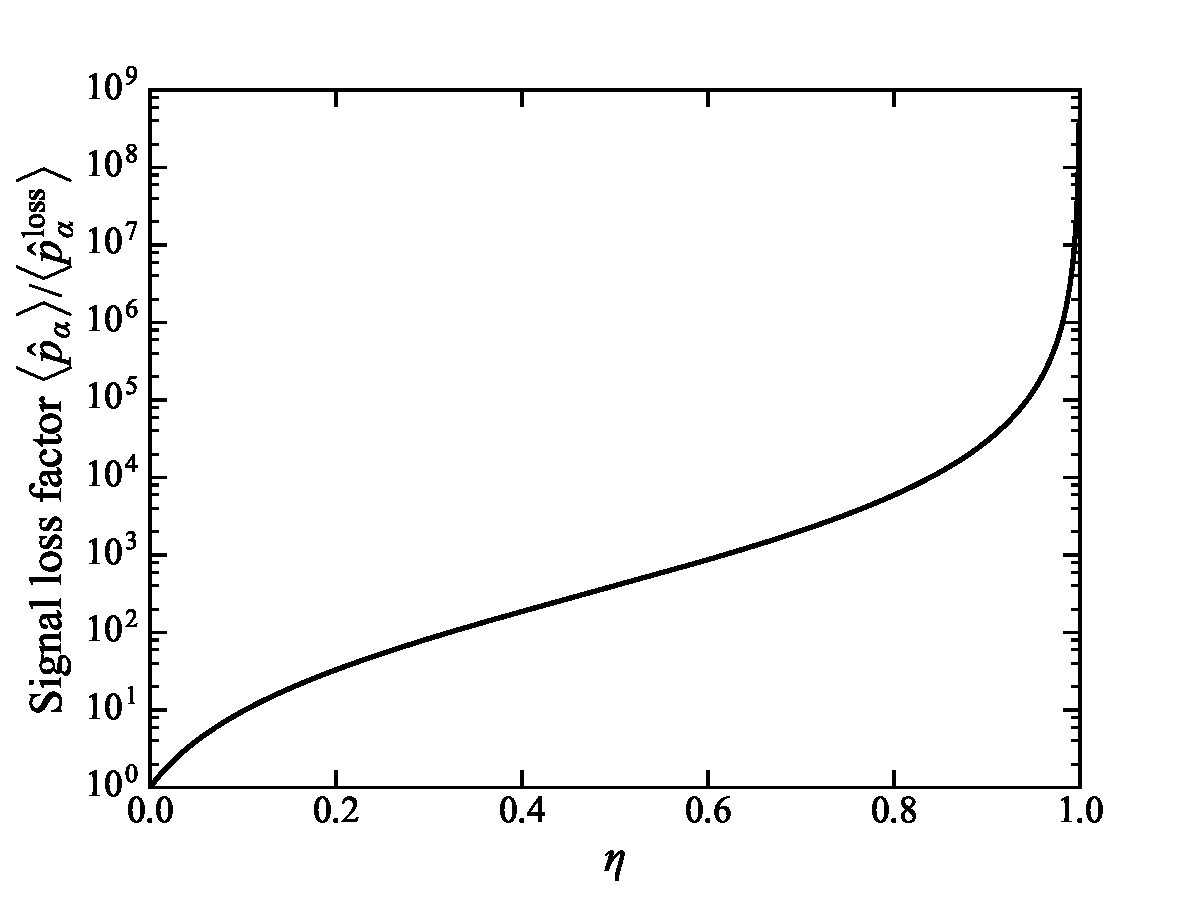
\includegraphics[width=0.6\columnwidth]{plots/analytic_sig_loss.pdf}
	\caption{Power spectrum signal loss for $N=20$ for a toy model where $\Chat = (1-\eta) \C + \eta \x \x^t$.}
	\label{fig:analytic_sig_loss}
\end{figure}

In general, one's estimate of the covariance will not be expressible in the form given by Eq. \eqref{eq:ChatDef}. However, the qualitative point here is that the signal loss can be expressed as a multiplicative factor. Even if $\Chat$ is more complicated than the form used for this toy model, the same mathematical technique of expressing the estimator as a series of higher-point functions, reducing these functions (assuming Gaussianity) to two-point functions, and re-summing any power series will show that the signal loss is a multiplicative factor. \acl{I can express this last bit more eloquently, but it's late and I'm tired and need to eat dinner.}


\bibliographystyle{apj}
\bibliography{refs}


\end{document}

